%%%%%%%%%%%%%%%%%%%%%%%%%%%%%%%%%%%%%%%%%%%%%%%%%%%%%%%%%%%%%%%%%%%%%%%%%%%%%%%%%
%
% This is a very basic template for mathematical presentations using LaTeX and beamer, aimed at University of Edinburgh students on the Honours Analysis course 2017-2018, for their "Skills" presentations.
%
% This template is just to get you started and to see what the possibilities are.  There is no required format, and you are free to use, discard, edit as much as you like.  I've put in some mathematical content to demonstrate the very basics of LaTeX.  Clearly, you will need to change this.
%
% Except for a few structural comments, I don't comment on the LaTeX itself.  If you have used it before, most of what you know should apply as usual.  If you have not, have a look at the source code, the output, and experiment with editing the code and see what happens.  Most LaTeX code is pretty intuitive, e.g. the command to produce an alpha is \alpha, the command for an integral sign is \int, etc.  You can learn an awful lot by guesswork, trial and error, and google.  
%
% The percent signs "%" are comment signs, and instruct LaTeX to ignore everything following the sign on the same line.  They can be used to comment on the code.
%
%%%%%%%%%%%%%%%%%%%%%%%%%%%%%%%%%%%%%%%%%%%%%%%%%%%%%%%%%%%%%%%%%%%%%%%%%%%%%%%%
%
% The following lines are the preamble.  They help LaTeX set-up the document, but do not print anything yet.

\documentclass{beamer}		% This tells LaTeX the document will be a "beamer" presentation

\usepackage{makecell}
\usepackage{tabularx}
\usepackage[export]{adjustbox}  
\usepackage{subcaption}

\usetheme{Madrid}		% Sets basic formatting.  Lots of options, google "beamer themes"
%
%\usetheme{Warsaw}

\usecolortheme{dolphin}	% Sets the colour scheme.  Lots of options, google "beamer color themes"

%\setbeamertemplate{navigation symbols}{}	% Manually changes one piece of formatting.  See what the difference is by commenting this line out.

\date{}	% Insert the date of your presentation. \today gives an unsurprising automatic date.

\title[]{A Decentralized PageRank Based\\Content Dissemination Model in the Edge of Network}	% Insert your title.  Depending on the theme you choose above, a "short title" might be useful, as it will appear on the footer of each slide.

\author[Xin Zhang]{Xin Zhang} % Insert your name

\institute[UCAS]{UCAS} % Self-explanatory
\date{\today}
\setbeamercovered{transparent}

\begin{document} 	% Let's begin

% Presentations come in slide frames.  You have to tell LaTeX when to start a frame, and when to end the frame.  The most common error beginners make with beamer is forgetting the \end{frame} command.	

\begin{frame}	
\titlepage	% Prints a title page populated with the information given in the preamble
\end{frame}		

\begin{frame}{Outline}
\begin{enumerate}[1. ]
    \item Introduction
    \item Related Works
    \item Content Dissemination Model
    \item Evaluation
    \item Future Work
    \item Conclusion
\end{enumerate}
\end{frame}



\begin{frame}{Outline}
\begin{enumerate}[1. ]
    \uncover<1>{\item Introduction}
    \uncover<>{\item Related Works}
    \uncover<>{\item Content Dissemination Model}
    \uncover<>{\item Evaluation}
    \uncover<>{\item Future Work}
    \uncover<>{\item Conclusion}
\end{enumerate}
\end{frame}

\begin{frame}{1. Introduction}
In order to improve the quality of content services, content is usually placed at the edge of the network which is close to users, such as CDN. In recent years, with the enhancement of edge device capabilities, it is hoped that more and more content will be placed on the wider edge including user devices and operator devices, such as set-top boxes, APs. Nevertheless, the traditional distribution methods are mostly based on centralized management. As the scale of edge devices growing larger, it will have a negative impact on the dissemination efficiency. Therefore, how to disseminate content in the edge of the network in a decentralized manner is an important issue.
\end{frame}

\begin{frame}{Outline}
\begin{enumerate}[1. ]
\uncover<>{\item Introduction}
\uncover<1>{\item Related Works}
\uncover<>{\item Content Dissemination Model}
\uncover<>{\item Evaluation}
\uncover<>{\item Future Work}
\uncover<>{\item Conclusion}
\end{enumerate}
\end{frame}

\begin{frame}{2. Related Work}
\begin{itemize}
    \item \textbf{Diffusion Models}
    \begin{itemize}
        \item Linear Threshold (LT) Model
        \item Independent Cascade (IC) Model
    \end{itemize}
\end{itemize}
\begin{itemize}
    \item \textbf{Existing Content Distribution Solutions}
    \begin{itemize}
        \item CDN
        \item Peer-to-peer
        \item Hybrid-P2P 
    \end{itemize}
\end{itemize}
\end{frame}

\begin{frame}{2. Related Work}
\framesubtitle{Diffusion Models}
\begin{itemize}
    \item Diffusion models were originally used in social networks to model the spread of influence in a network.
    \item The Susceptible-Infected-Recovered (SIR) model is the most classic information diffusion model.
    \item In these models each node is either active or inactive. Over iterations an inactive node becomes active as more of its neighbors become active. The two most popular diffusion models are the linear threshold model and the independent cascade model.
    \item The two most popular diffusion models are:
    \begin{itemize}
        \item Linear threshold (LT) model
        \item Independent cascade (IC) model
    \end{itemize} 
\end{itemize}
\end{frame}

\begin{frame}{2. Related Work}
\framesubtitle{Diffusion Models}
\begin{description}
\item[LT Model] Each edge has an activation probability and the influence is propagated by activated nodes independently activating their inactive neighbors based on the edge activation probabilities. 
\end{description}
\begin{description}
\item[IC Model] Each edge has a weight, each vertex has threshold chosen uniformly at random, and a vertex becomes activated if the weighted sum of its active neighbors exceeds its threshold.
\end{description}
\begin{block}{Neither of the above two solutions can be used}
\begin{itemize}
    \item Application scenarios of the above two diffusion models are different from the self-diffusion scenario of the home router cluster of the community network in this paper.
    \begin{itemize}
        \item It is hoped that the content will be distributed evenly in the network.
        \item However, in the above two models, only after enough neighbor nodes have cached the content, the current node is willing to cache the content. This can lead to uneven distribution of the content. 
    \end{itemize}
\end{itemize}
\end{block}
\end{frame}

\begin{frame}{2. Related Work}
\framesubtitle{Existing Content Distribution Solutions - \textcolor{red}{CDN}}
\begin{block}{CDN}
A CDN is a geographically distributed network of proxy servers and their data centers.
Three mechanisms are as follows:
\end{block}
\begin{description}
    \item[Pull-based] Dispatching user requests to appropriate edge nodes. If the current node does not have the content required by the user, the layer-by-layer query is performed upwards. 
    \item[Push-based] Replicating objects on certain servers in advance, namely deciding how to pre-deploy the content based on the analysis on the user behavior.
    \item[Hybrid] First half of which is a pre-deployment via a push-based mechanism, and the latter half is based on a pull-based mechanism. In fact, YouTube, as the largest online video-sharing service, keeps employing CDNs to deliver its most popular videos to its users.
\end{description}
\end{frame}

\begin{frame}{2. Related Work}
\framesubtitle{Existing Content Distribution Solutions - \textcolor{red}{Peer-to-peer}}
\begin{block}{Peer-to-peer}
Peer-to-peer (P2P) computing or networking is a distributed application architecture that partitions tasks or workloads between peers, without the need for central coordination by servers or stable hosts.P2P media streaming aims at utilizing the uploading bandwidth of the clients. Two mainstream architectures have been devised: 
\end{block}
\begin{description}
    \item[Tree-based push] The tree-based system acts as a natural extension of CDNs. Instead of only having two layers of the client-server structure, it has many such layers by allowing every client to become a potential server to some other clients.
    \item[Mesh-based pull] Unlike the tree-based push system, the mesh-based system requires peers to share the information about their media repository, which guides a peer to pull its desired media chunk from others.
\end{description}
\end{frame}

\begin{frame}{2. Related Work}
\framesubtitle{Existing Content Distribution Solutions - \textcolor{red}{Hybrid-p2p}}
\begin{block}{Hybrid-p2p}
Hybrid P2P systems are a combination of peer-to-peer and client-server models. 
\end{block}
\begin{itemize}
\item Servers in CDNs are organized in a tree structure, which consists of, from top to bottom, the source server owned by content providers, core service nodes, and edge ones. Each edge service node serves end users that are usually in the same ISP.
\item  Clients form a tree-mesh combined overlay to forward the received streams.
\end{itemize}
\end{frame}

\begin{frame}{2. Related Work}
\framesubtitle{What's New in Our Model}
Different from the existing methods, a \textbf{self-diffusion} process is added into the home router cluster in the edge of network to better assist the video distribution and offline downloading.
\begin{itemize}
    \item The application scenario of this paper is how to make edge devices such as home routers, instead of operator servers in the traditional sense, work together to pre-deploy the content to enhance the content service performance.
    \item In our scenario, the framework is similar to the existing CDN-P2P model.
\end{itemize}
\end{frame}

\begin{frame}{Outline}
\begin{enumerate}[1. ]
\uncover<>{\item Introduction}
\uncover<>{\item Related Works}
\uncover<1>{\item Content Dissemination Model}
\uncover<>{\item Evaluation}
\uncover<>{\item Future Work}
\uncover<>{\item Conclusion}
\end{enumerate}
\end{frame}

\begin{frame}{3. Content Dissemination Model}
\begin{itemize}
\item \textbf{Statement}
\item \textbf{Decentralized Content Dissemination Algorithm (DCDM)}
\item \textbf{Decentralized Weighted PageRank-style Node Selection Algorithm}
\begin{itemize}
    \item PageRank
    \item Weighted PageRank
    \item Parameters Approximation
\end{itemize}
\end{itemize}
\end{frame}

\begin{frame}{3. Content Dissemination Model}
\framesubtitle{Statement}
The application scenario in this paper is the community network, where each node is embodied as a home router. Every node is aware of the following information:
\[<nodeId,peerList,fileState,curCov,needCov,bandwidth>\]
\begin{itemize}
    \item \textcolor{red}{\(nodeId\)} is the ID of the node.
    \item \textcolor{red}{\(fileState\)} records the file status on the current node.
    \item \textcolor{red}{\(curCov\)} is the current coverage rate of the specific file.
    \item \textcolor{red}{\(needCov\)} represents the expected coverage rate.
    \item \textcolor{red}{\(bandwidth\)} represents the rate of data transfer.
\end{itemize}
\end{frame}

\begin{frame}{3. Content Dissemination Model}
\framesubtitle{Decentralized Content Dissemination Algorithm (DCDM)}
Each node has at least a certain number of neighbors with good link connectivity. Five steps:
\begin{columns}
\column{0.5\textwidth}
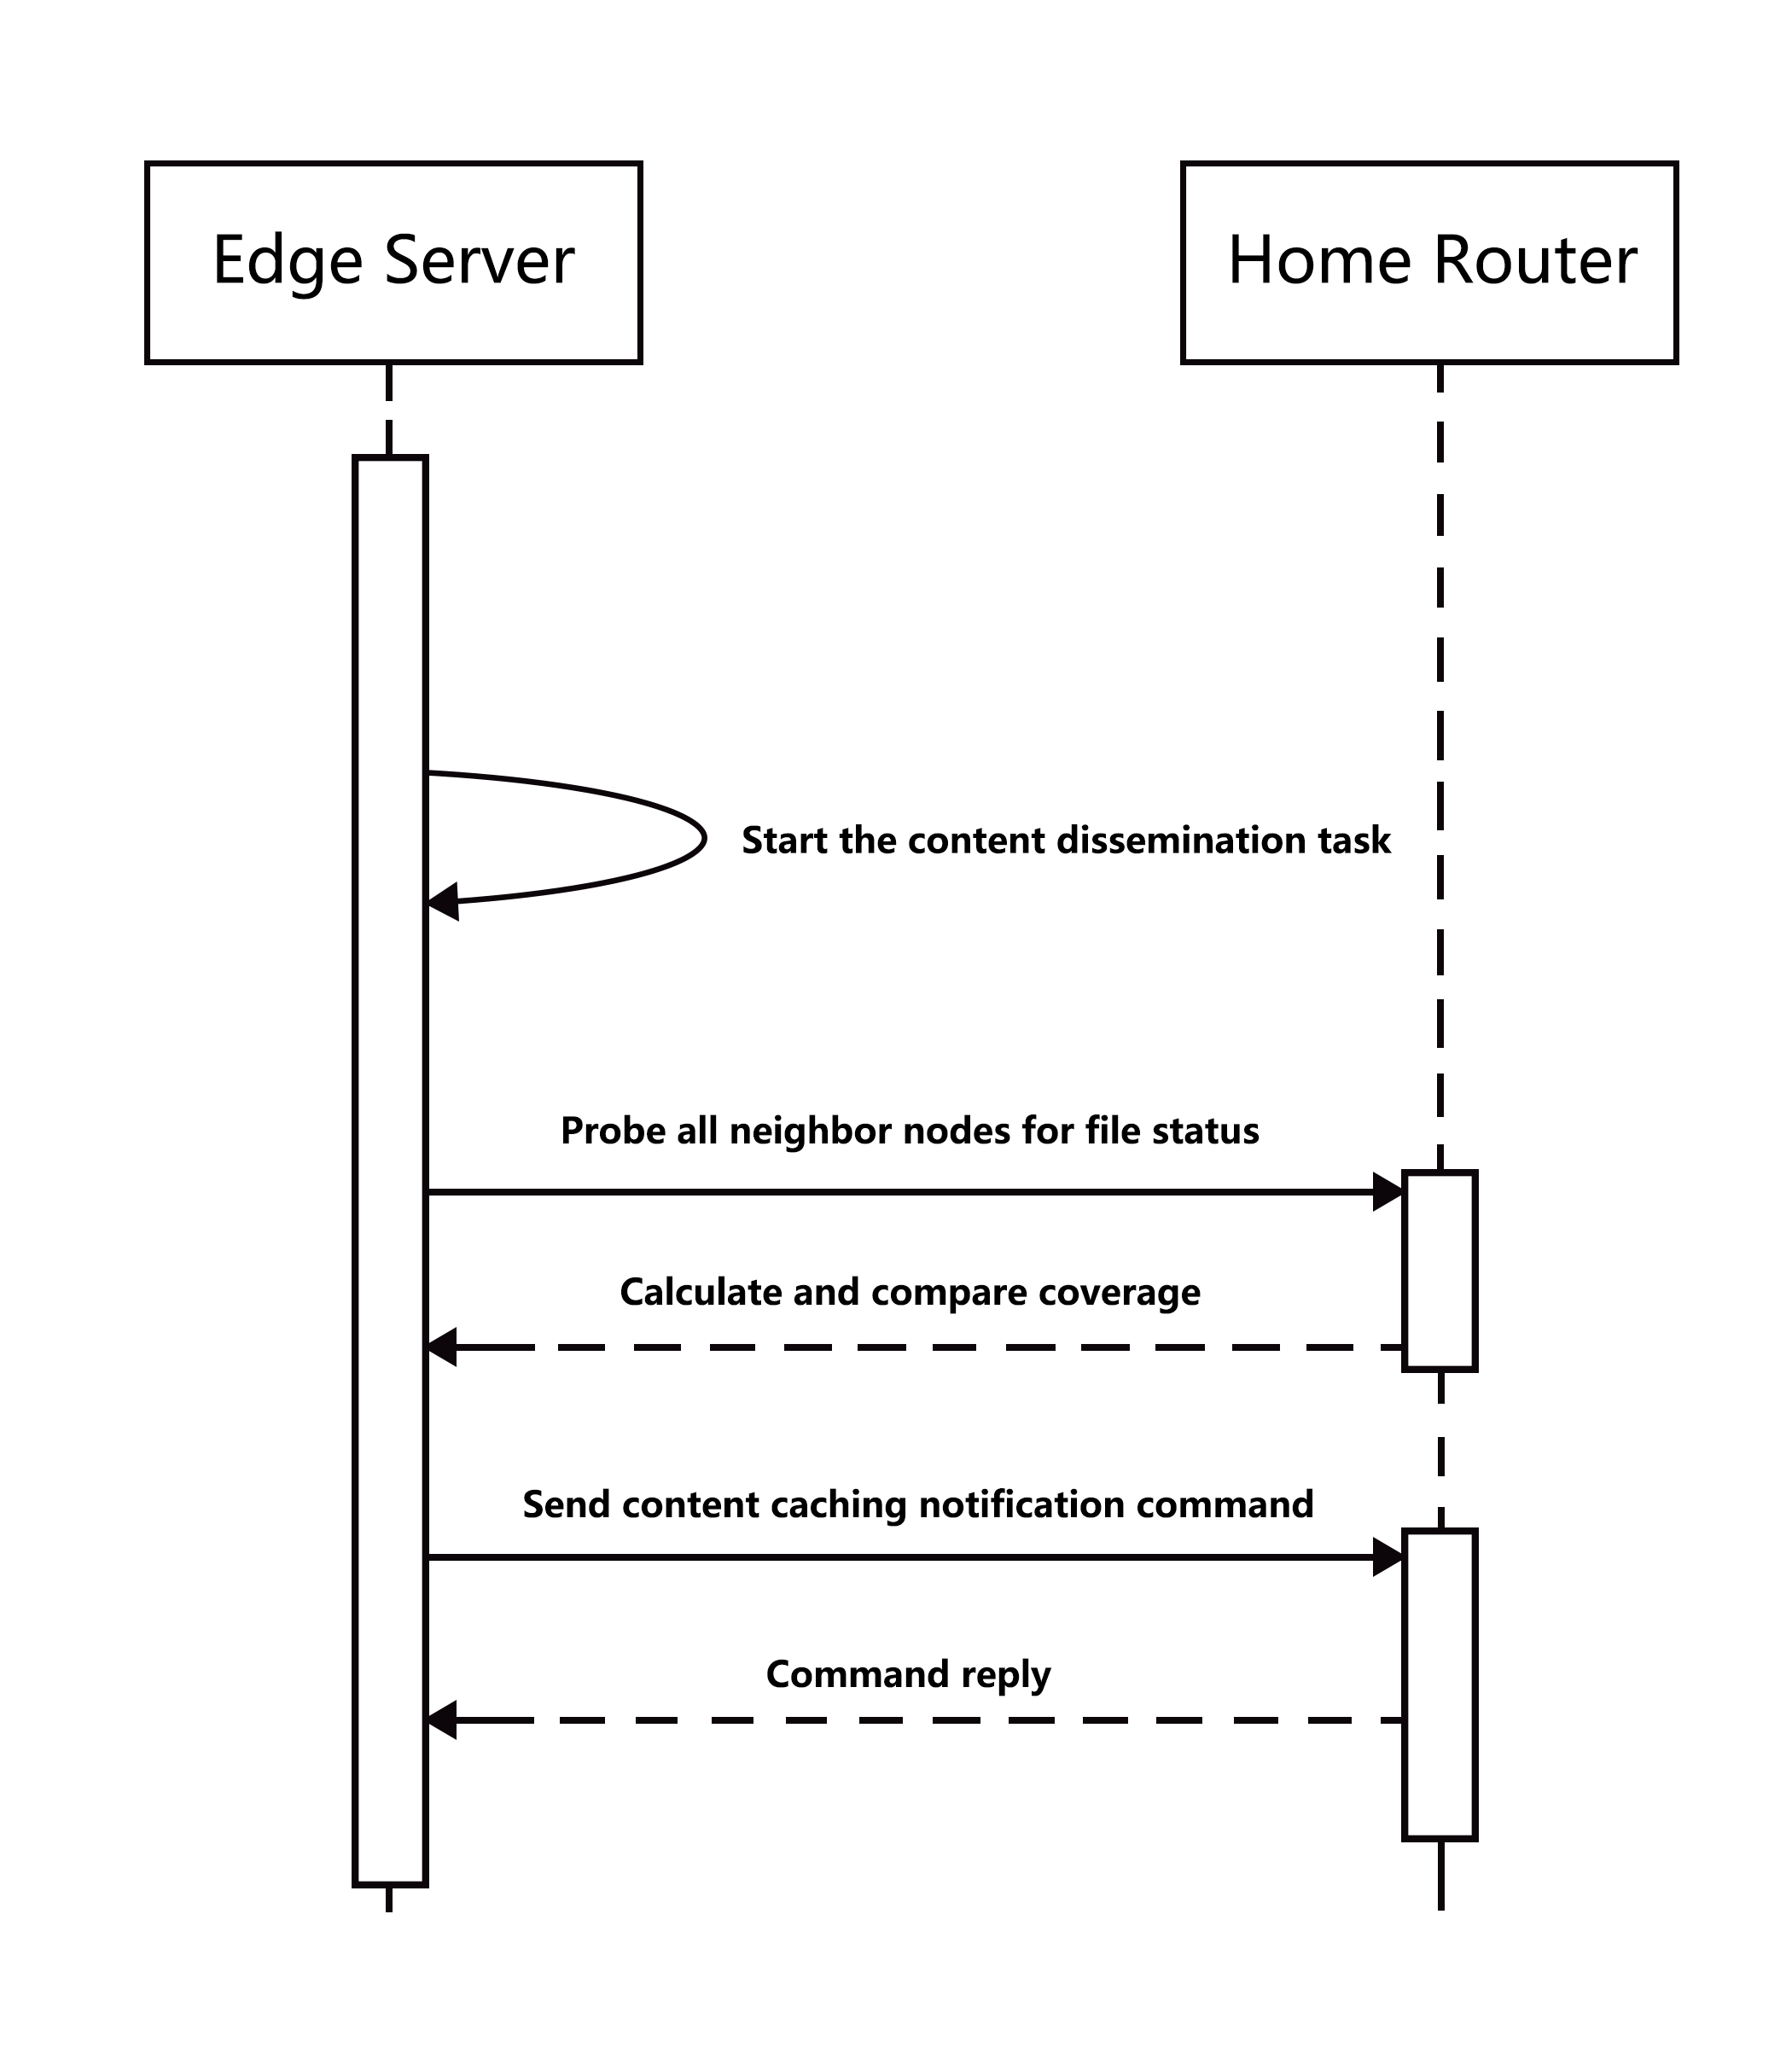
\includegraphics[scale=0.08]{imgs/Figure1.png}
\column{0.5\textwidth}
\begin{enumerate}
    \item[1.] Once the content dissemination task starts, the edge server probes all neighbor nodes for file status.
    \item[2.] then calculates the current coverage and compares it with the requirement.
    \item[3.] If not reached, the node selection algorithm is used to rank neighbors and select the appropriate ones with a certain coverage rate.
\end{enumerate}
\end{columns}
\end{frame}

\begin{frame}{3. Content Dissemination Model}
\framesubtitle{Decentralized Content Dissemination Algorithm (DCDM)}
\begin{columns}
\column{0.5\textwidth}
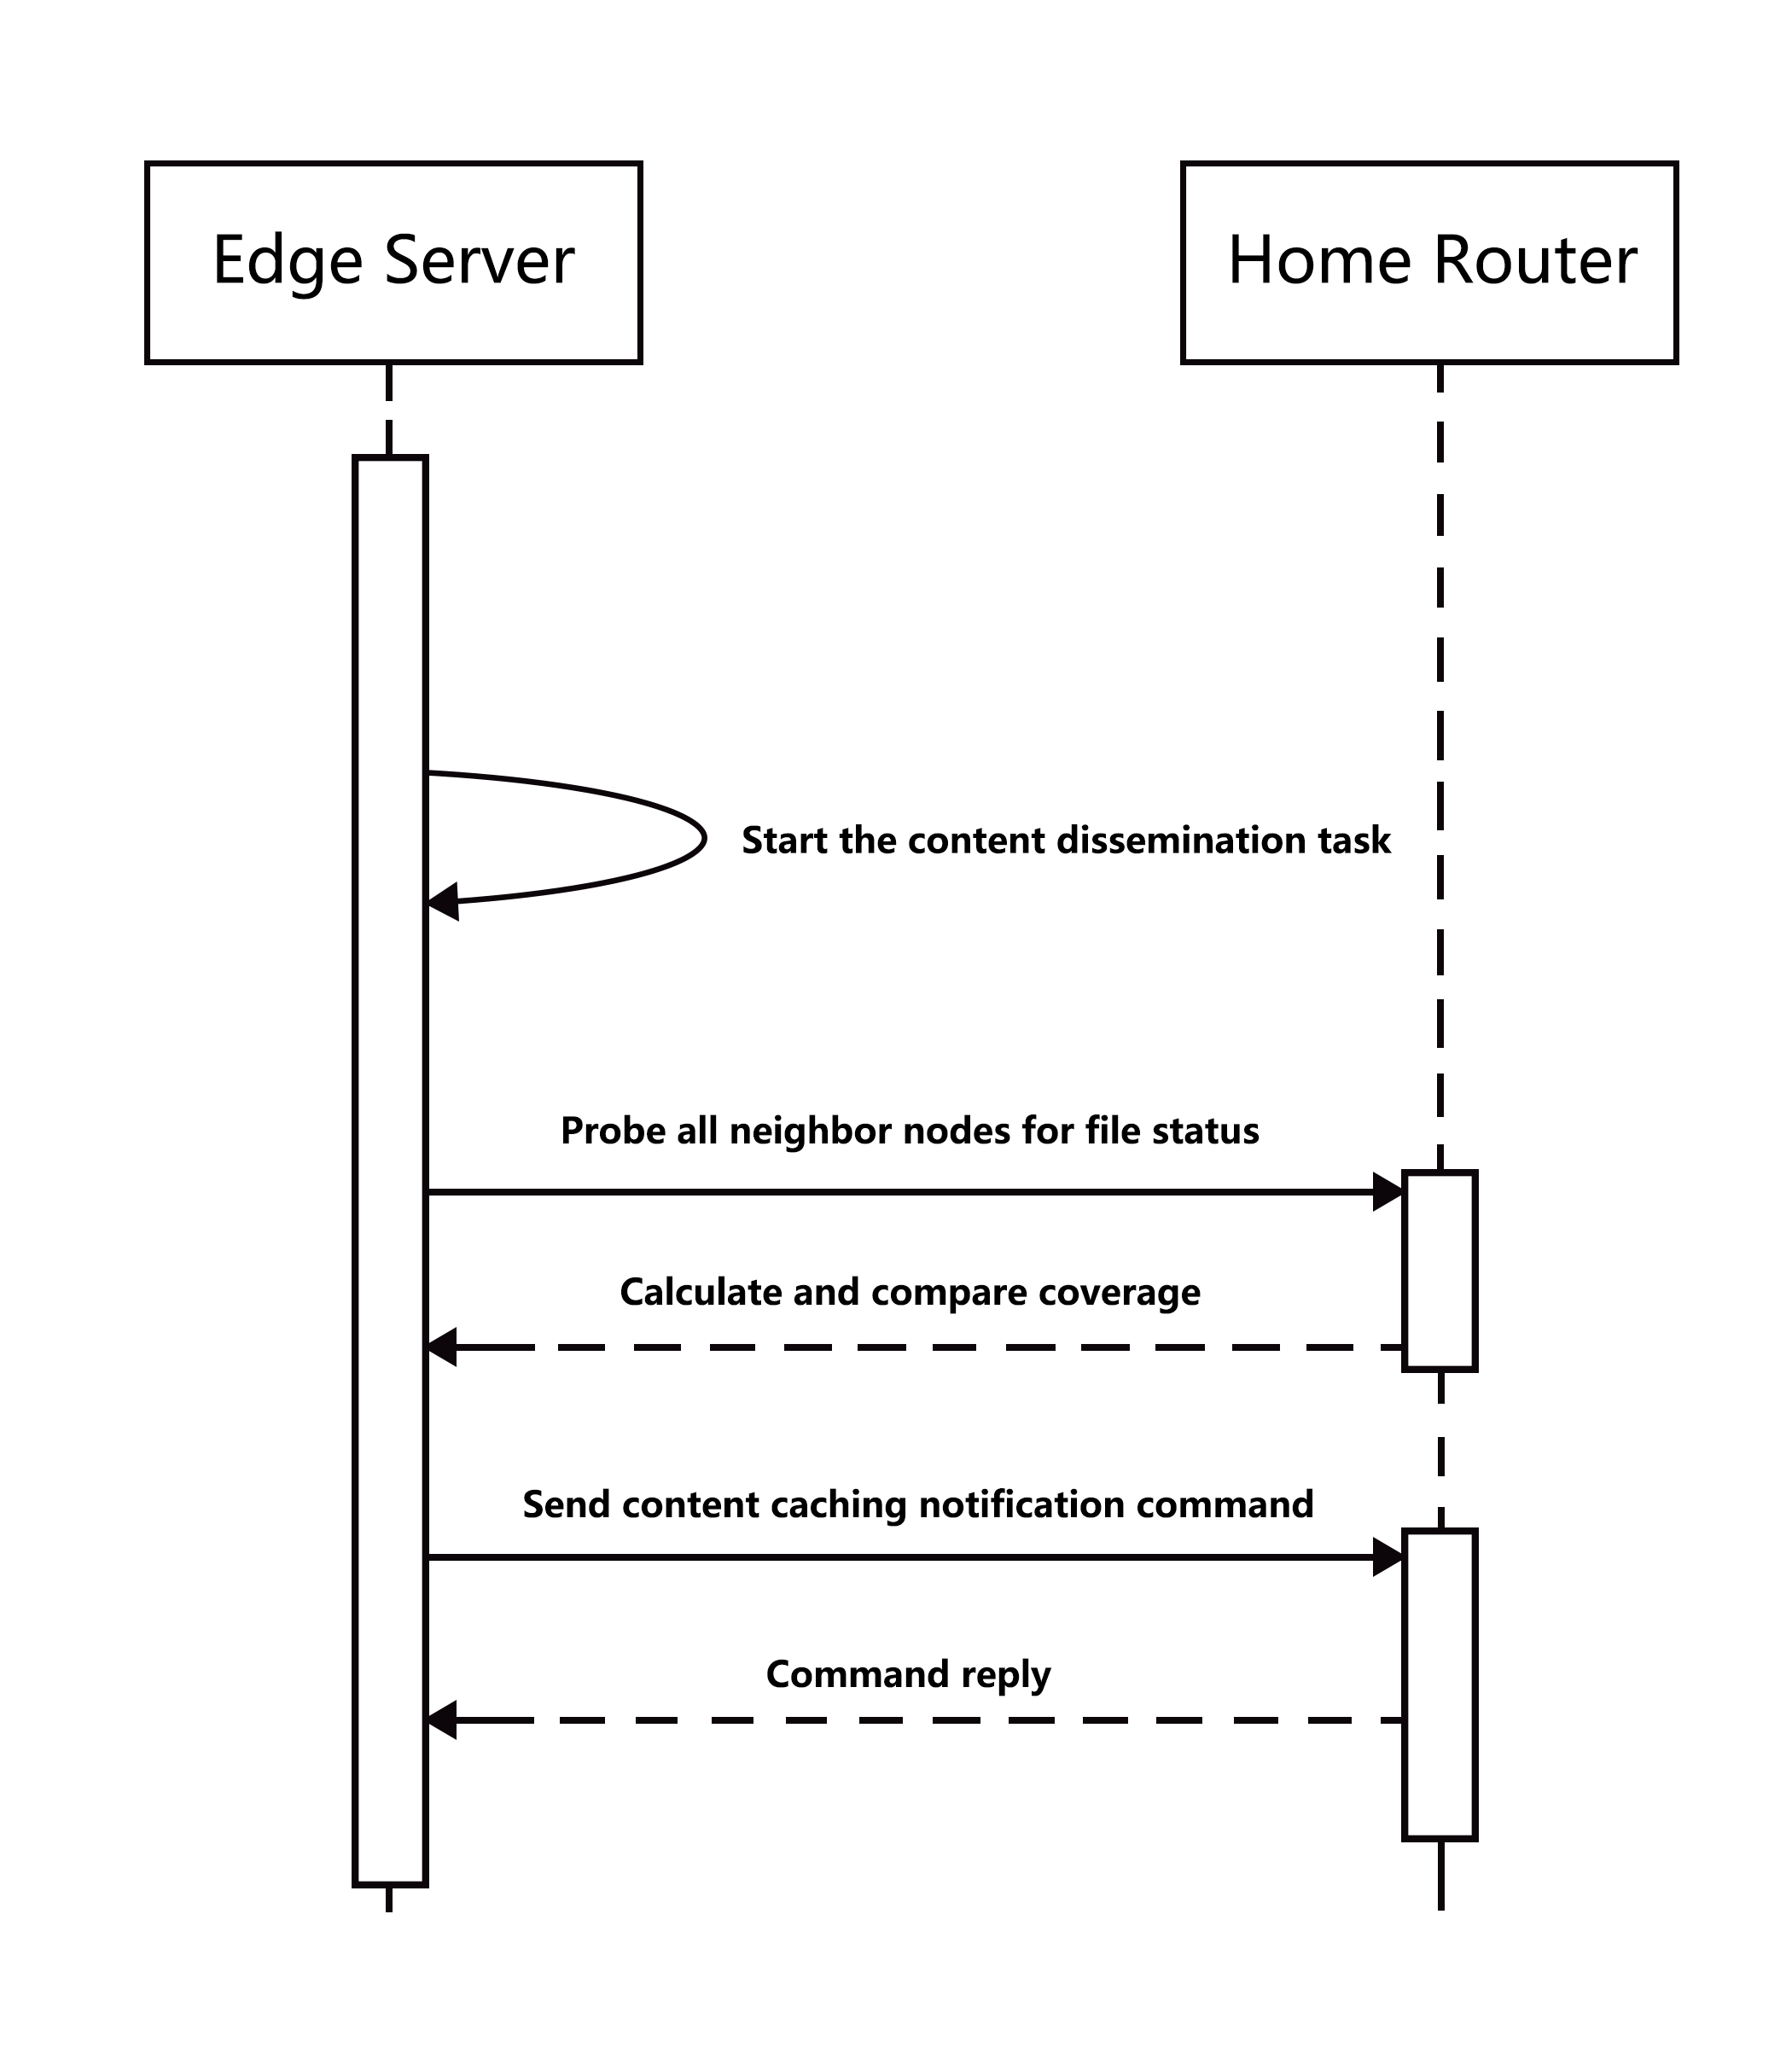
\includegraphics[scale=0.08]{imgs/Figure1.png}
\column{0.5\textwidth}
\begin{enumerate}
    \item[4.] A content caching notification command will be sent to neighbors selected by the node selection algorithm.
    \item[5.] When the ratio of neighbor nodes owning content reaches or exceeds the default coverage requirement, or there are no more quotas, the current node has already completed the dissemination step.
\end{enumerate}
\end{columns}
\end{frame}

\begin{frame}
\frametitle{3. Content Dissemination Model}
\framesubtitle{Decentralized Content Dissemination Algorithm (DCDM)}
\begin{figure}[t]
    \centering
    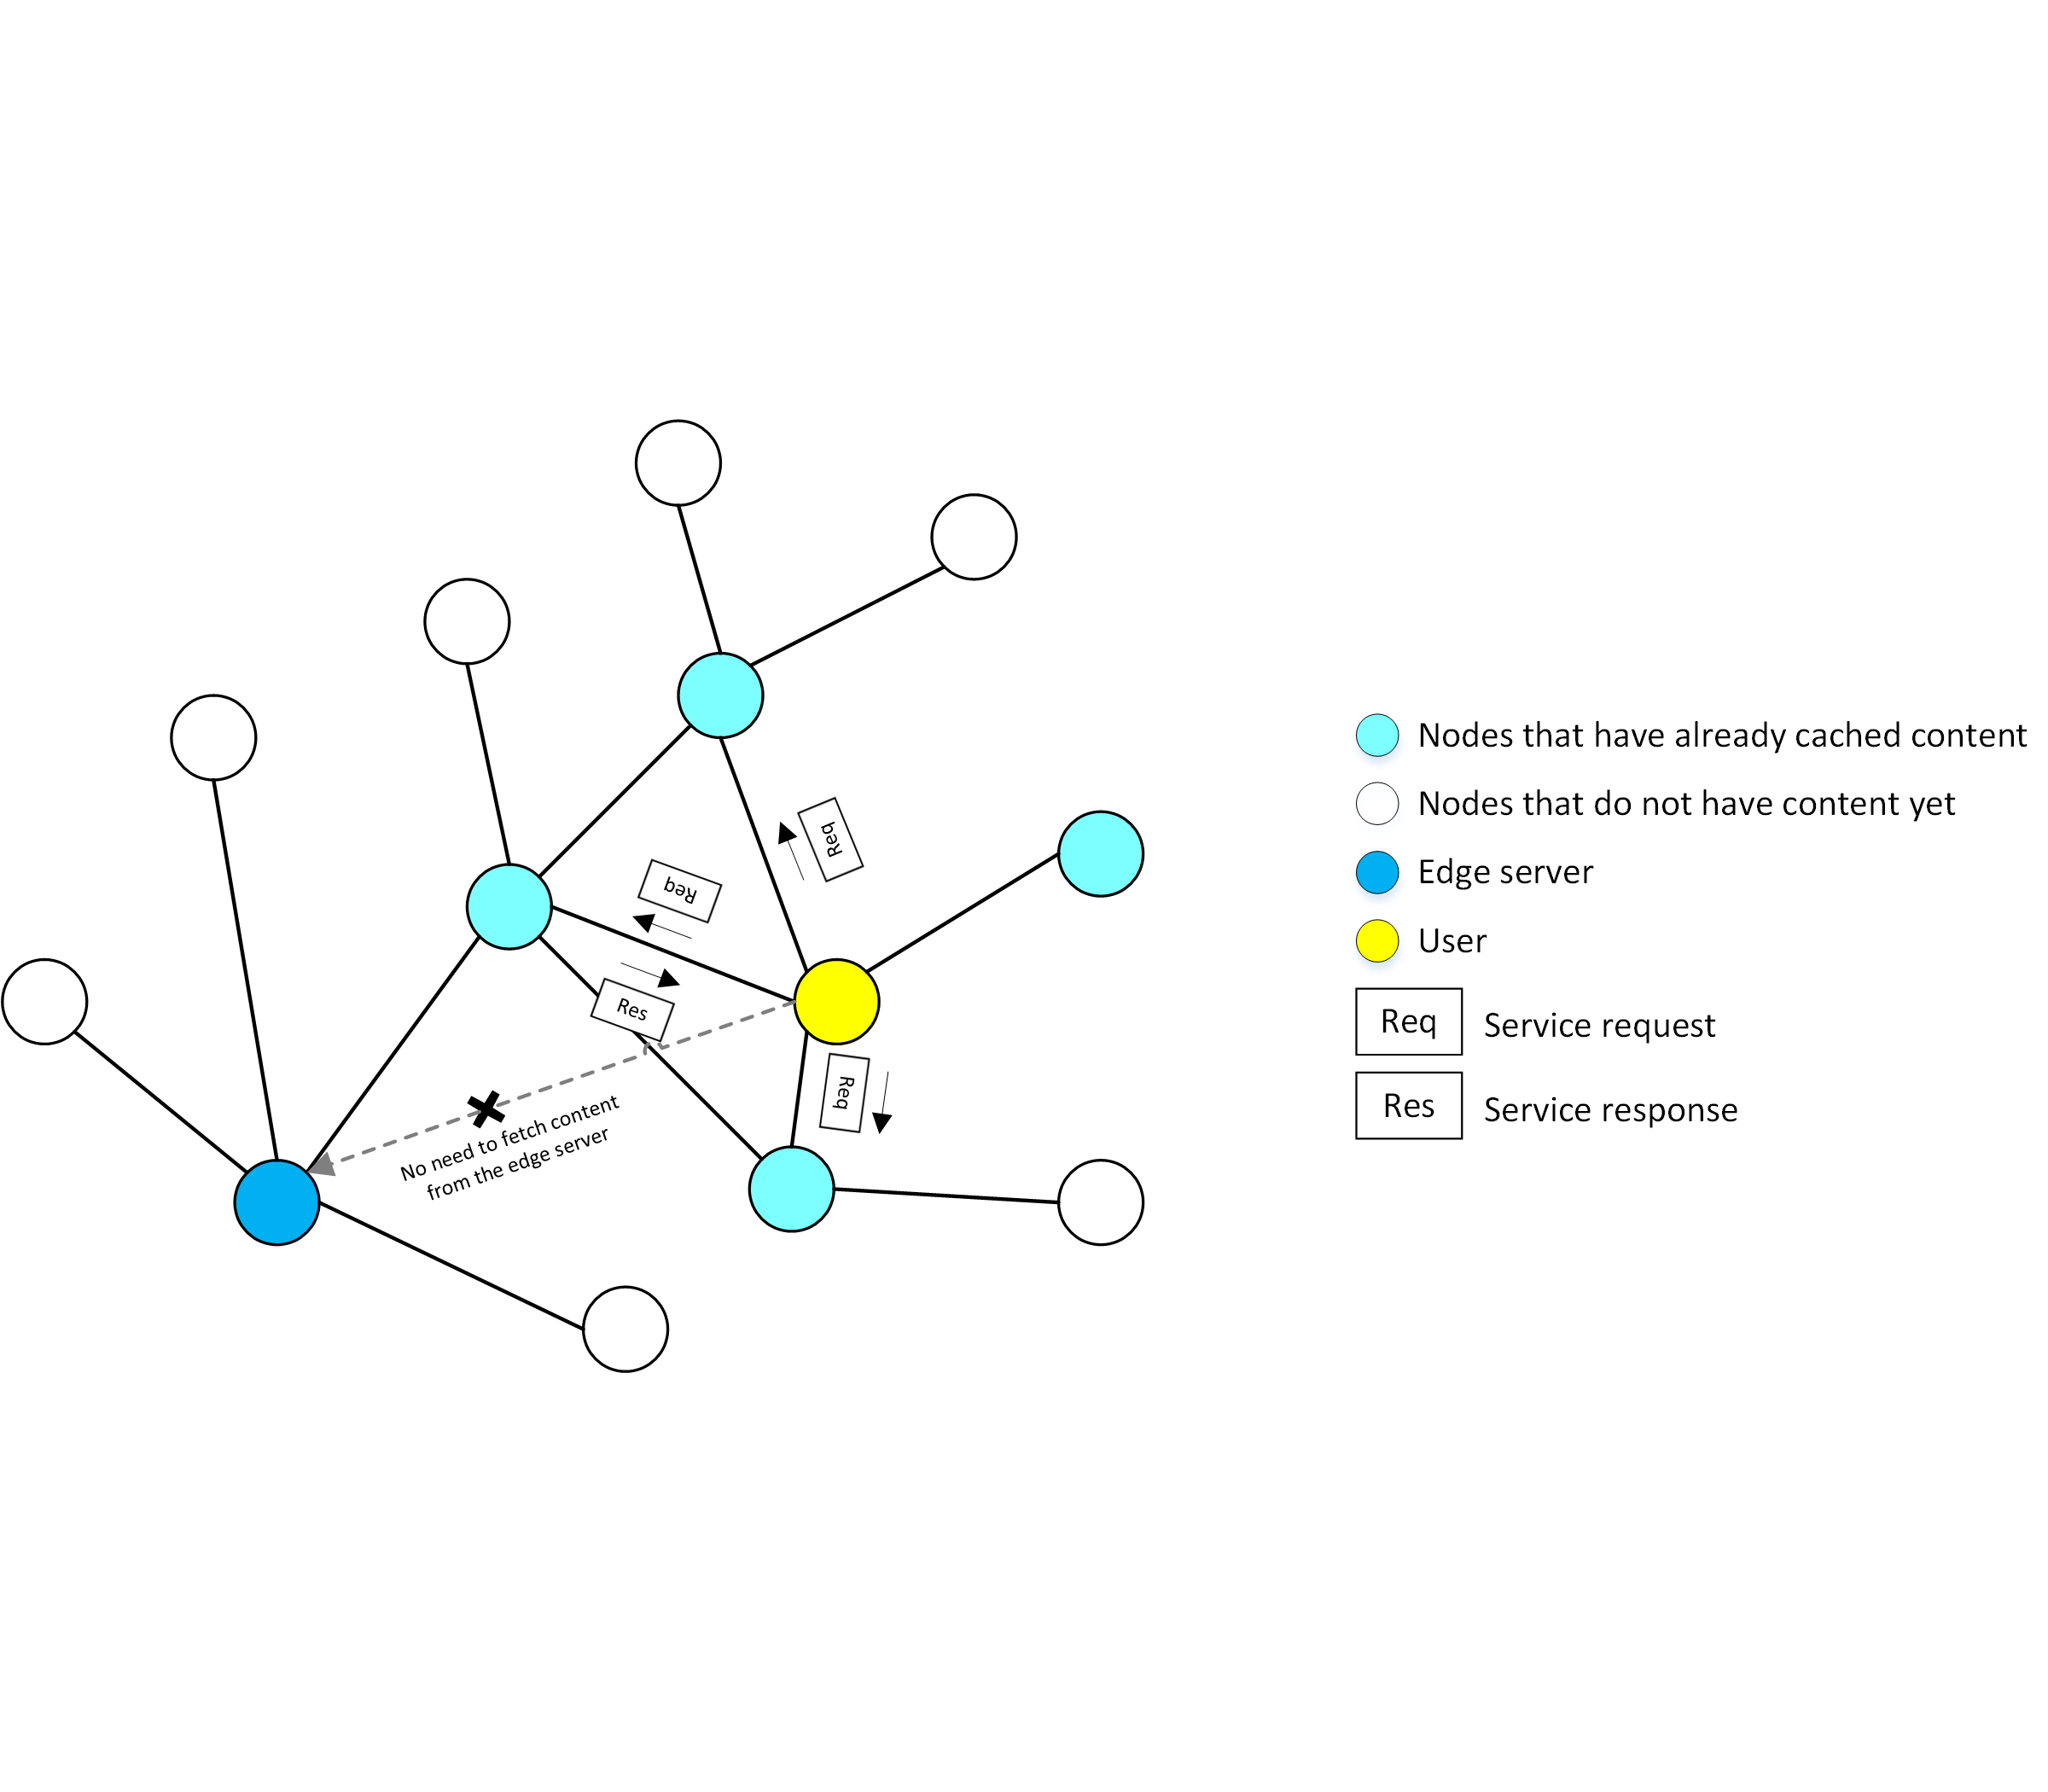
\includegraphics[width=0.6\textwidth]{imgs/Figure2.png}
    \caption{Network Diagram}
\end{figure}
\end{frame}

\begin{frame}{3. Content Dissemination Model}
\framesubtitle{Decentralized Content Dissemination Algorithm (DCDM)}
\begin{columns}
\column{0.5\textwidth}
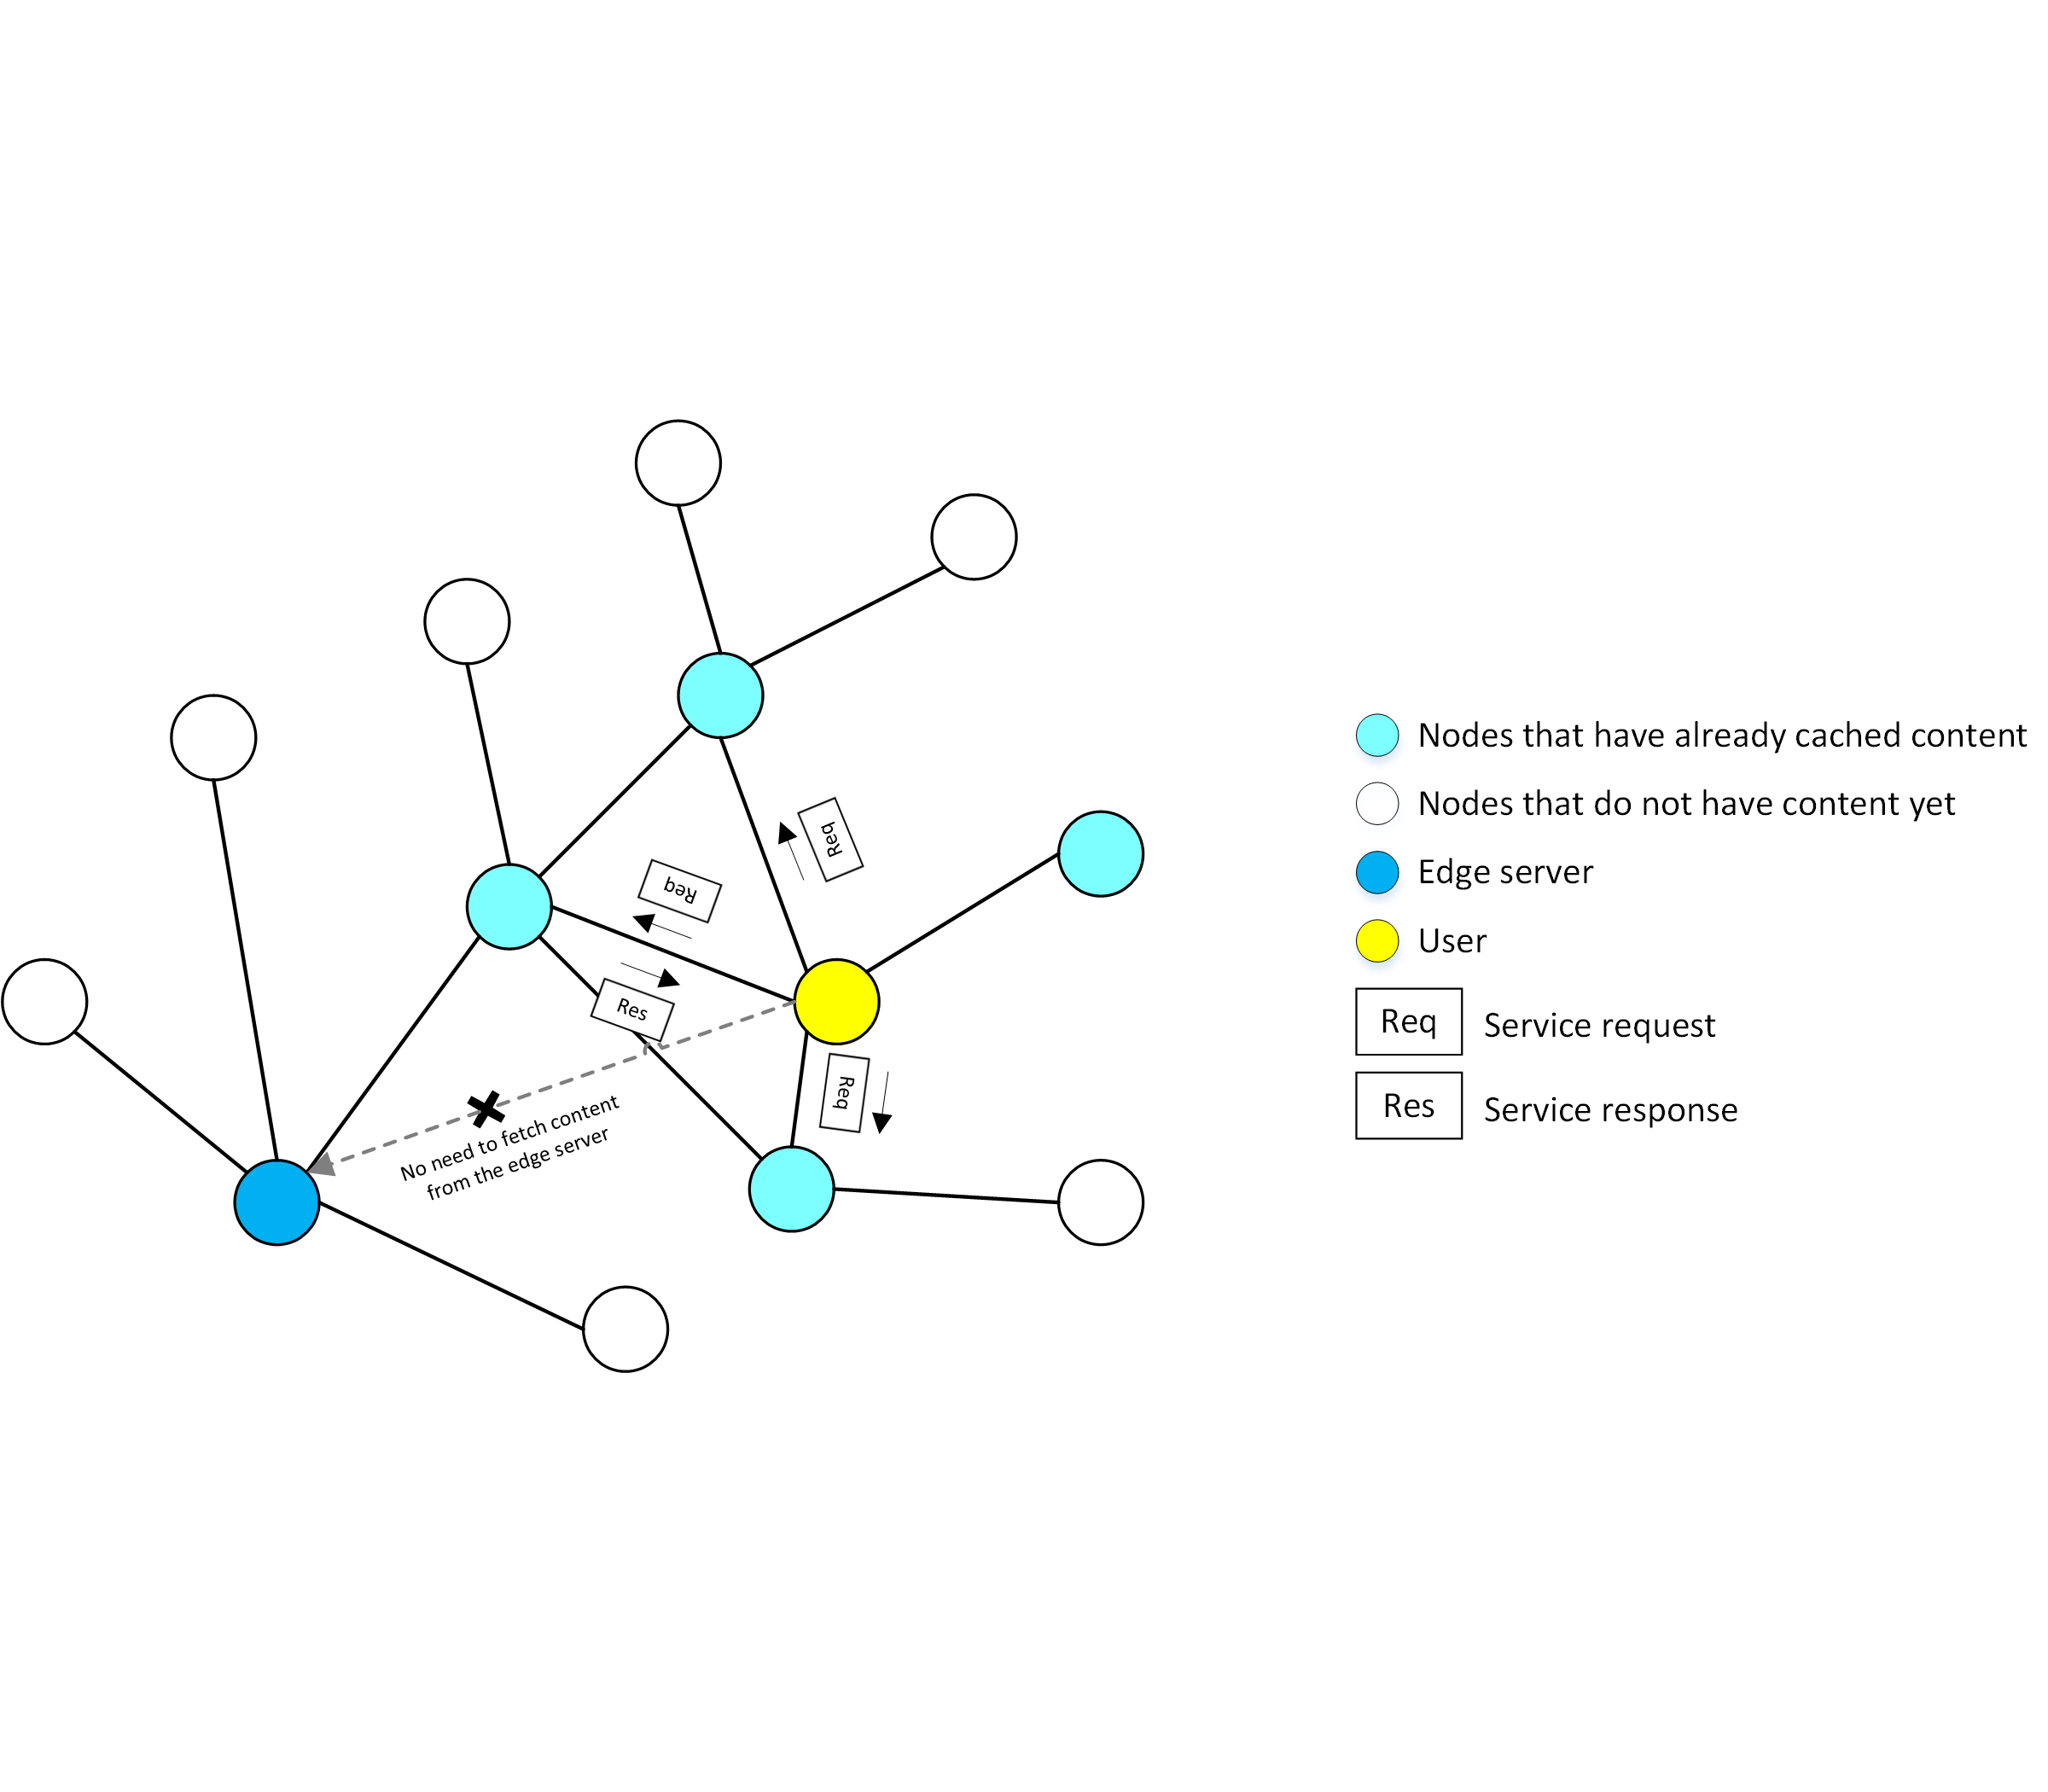
\includegraphics[scale=0.07]{imgs/Figure2.png}
\column{0.5\textwidth}
\begin{itemize}
    \item Each node has a certain number of neighbors, some of which have already cached content. 
    \item Twenty percent of nodes are randomly selected as users. 
    \item User requests obey Poisson distribution.
    \item When there is a user request, the user can directly obtain data from neighbor nodes without obtaining from a remote edge server.
\end{itemize}
\end{columns}
\end{frame}

\begin{frame}{3. Content Dissemination Model}
\framesubtitle{Decentralized Weighted PageRank-style Node Selection Algorithm}
Because the node selection algorithm is the most important part of the entire model, a decentralized weighted PageRank-style node selection algorithm is proposed, which is based on the following thoughts. The content should be cached on nodes as follows:
\begin{itemize}
    \item Firstly, nodes with a central position.
    \item Secondly, nodes with high bandwidth and low-latency network connections, which are able to support QoS requirements. 
    \item Thirdly, nodes that are close to users, from the perspective of hops, etc.
\end{itemize}
\end{frame}

\begin{frame}{3. Content Dissemination Model}
\framesubtitle{Decentralized Weighted PageRank-style Node Selection Algorithm - \textcolor{red}{PageRank}}
PageRank is a link algorithm assessing the importance of web pages. The fundamental idea is that the importance of a node is judged by the number of nodes linking to it as well as their importance.
\[
PR(P_i)=\frac{1-\alpha}{N}+\alpha\sum_{P_j\in B_i}{\frac{PR(P_j)}{l_j}}
\]
where $B_i$ denotes a collection of nodes pointing to $P_i$, $l_j$ denotes the number of outgoing links of $P_j$, $N$ denotes the total number of nodes, and $\alpha$ denotes the damping factor, with $0<\alpha<1$ and usually set to a value around 0.85. With probability , a surfer chooses the next node at random.
\end{frame}

\begin{frame}{3. Content Dissemination Model}
\framesubtitle{Decentralized Weighted PageRank-style Node Selection Algorithm - \textcolor{red}{Weighted PageRank}}
In a directed weighted complex network with $n$ nodes, for node $v$, links to node $v$ are denoted by $v_1,v_2,\dots,v_l$, the corresponding weights are denoted by $\omega(v_i,v)$ where $1\leq i\leq l$. Then the calculation formula of weighted PageRank is derived as follows:
\begin{equation}
\begin{aligned}
PR(v)&=\frac{1-\alpha}{n}+\alpha(\frac{\omega(v_1,v)}{S_{out}(v_1)})PR(v_1)+\dots+\frac{\omega(v_l,v)}{S_{out}(v_l)})PR(v_l)\\
&=\frac{1-\alpha}{n}+\alpha\sum_{i=1}^l\frac{\omega(v_i,v)}{\sum_{j=1}^{m_i}\omega(v_i,z_j)}PR(v_i)
\end{aligned}
\end{equation}
\begin{block}{New Weighting Scheme}
This new weighting scheme does not only evaluate the topological position of a node, but also its network and hardware resources.
\end{block}
\end{frame}{}

\begin{frame}{3. Content Dissemination Model}
\framesubtitle{Decentralized Weighted PageRank-style Node Selection Algorithm - \textcolor{red}{Parameters Approximation}}
\begin{figure}
    \centering
    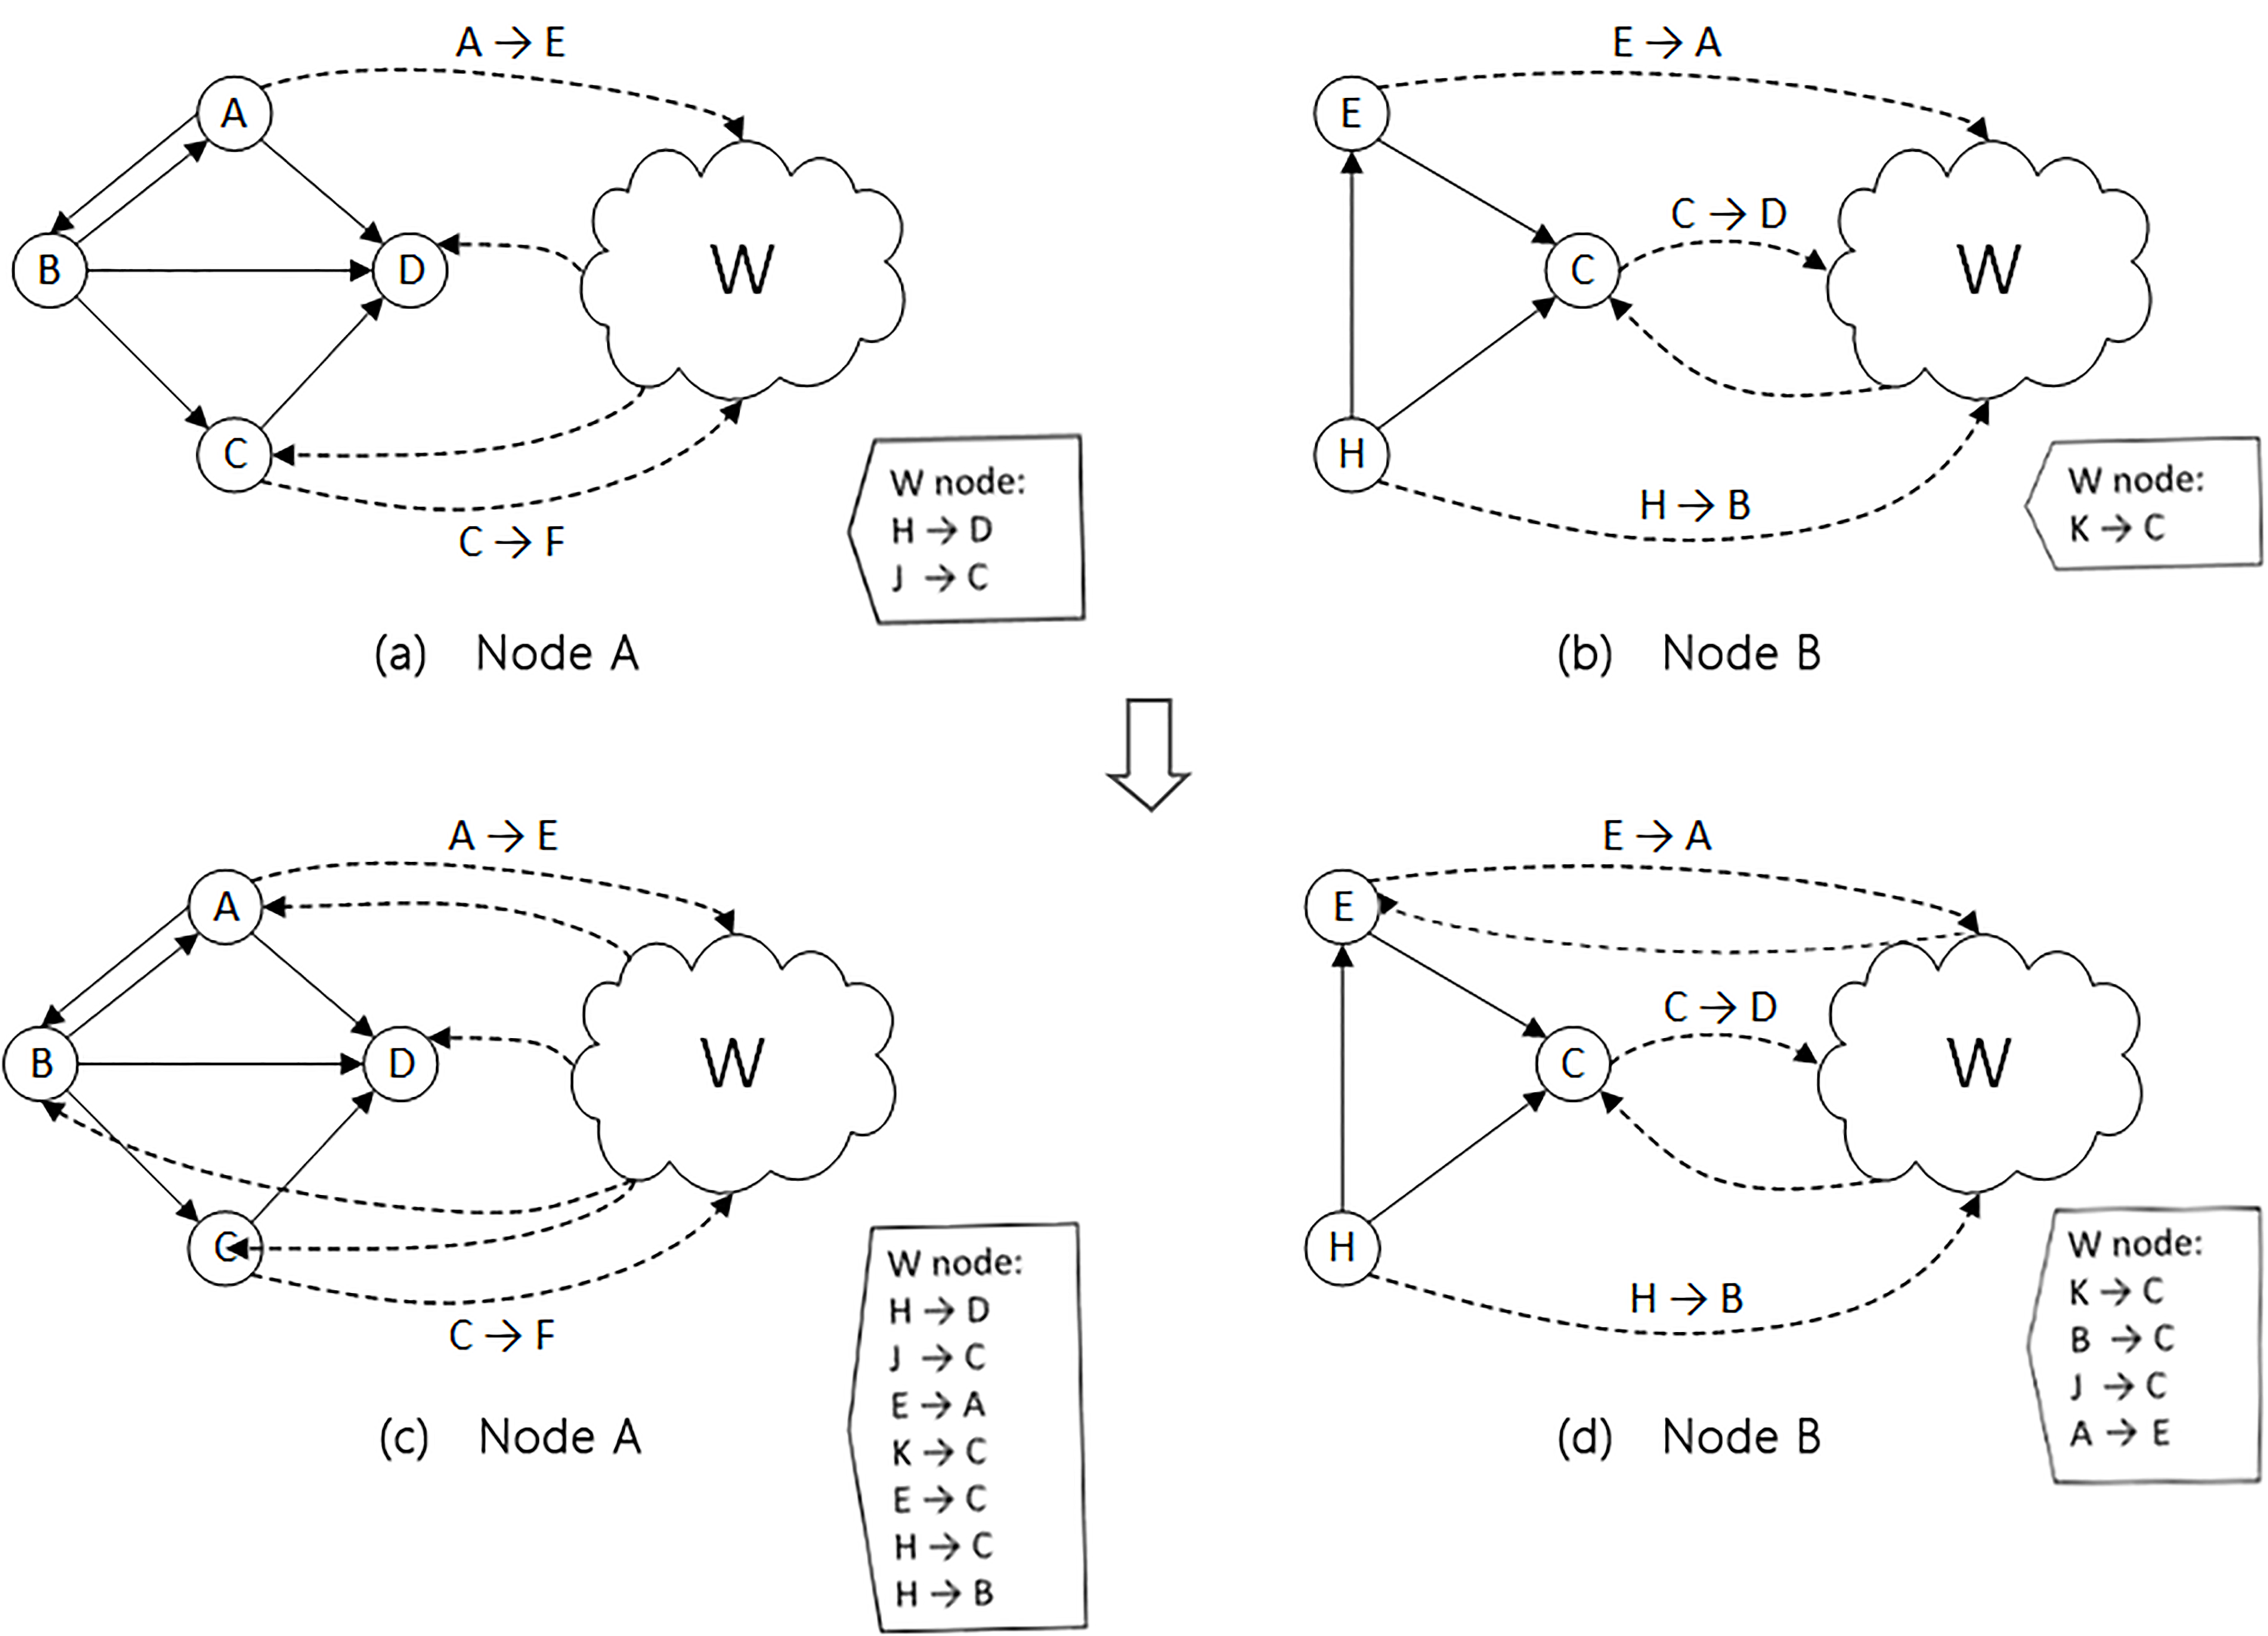
\includegraphics[width=0.7\textwidth]{imgs/Fig3.png}
    \caption{Demonstration of the light-weight merging phase}
\end{figure}
\end{frame}

\begin{frame}{3. Content Dissemination Model}
\framesubtitle{Decentralized Weighted PageRank-style Node Selection Algorithm - \textcolor{red}{Parameters Approximation}}
\begin{columns}
\column{0.5\textwidth}
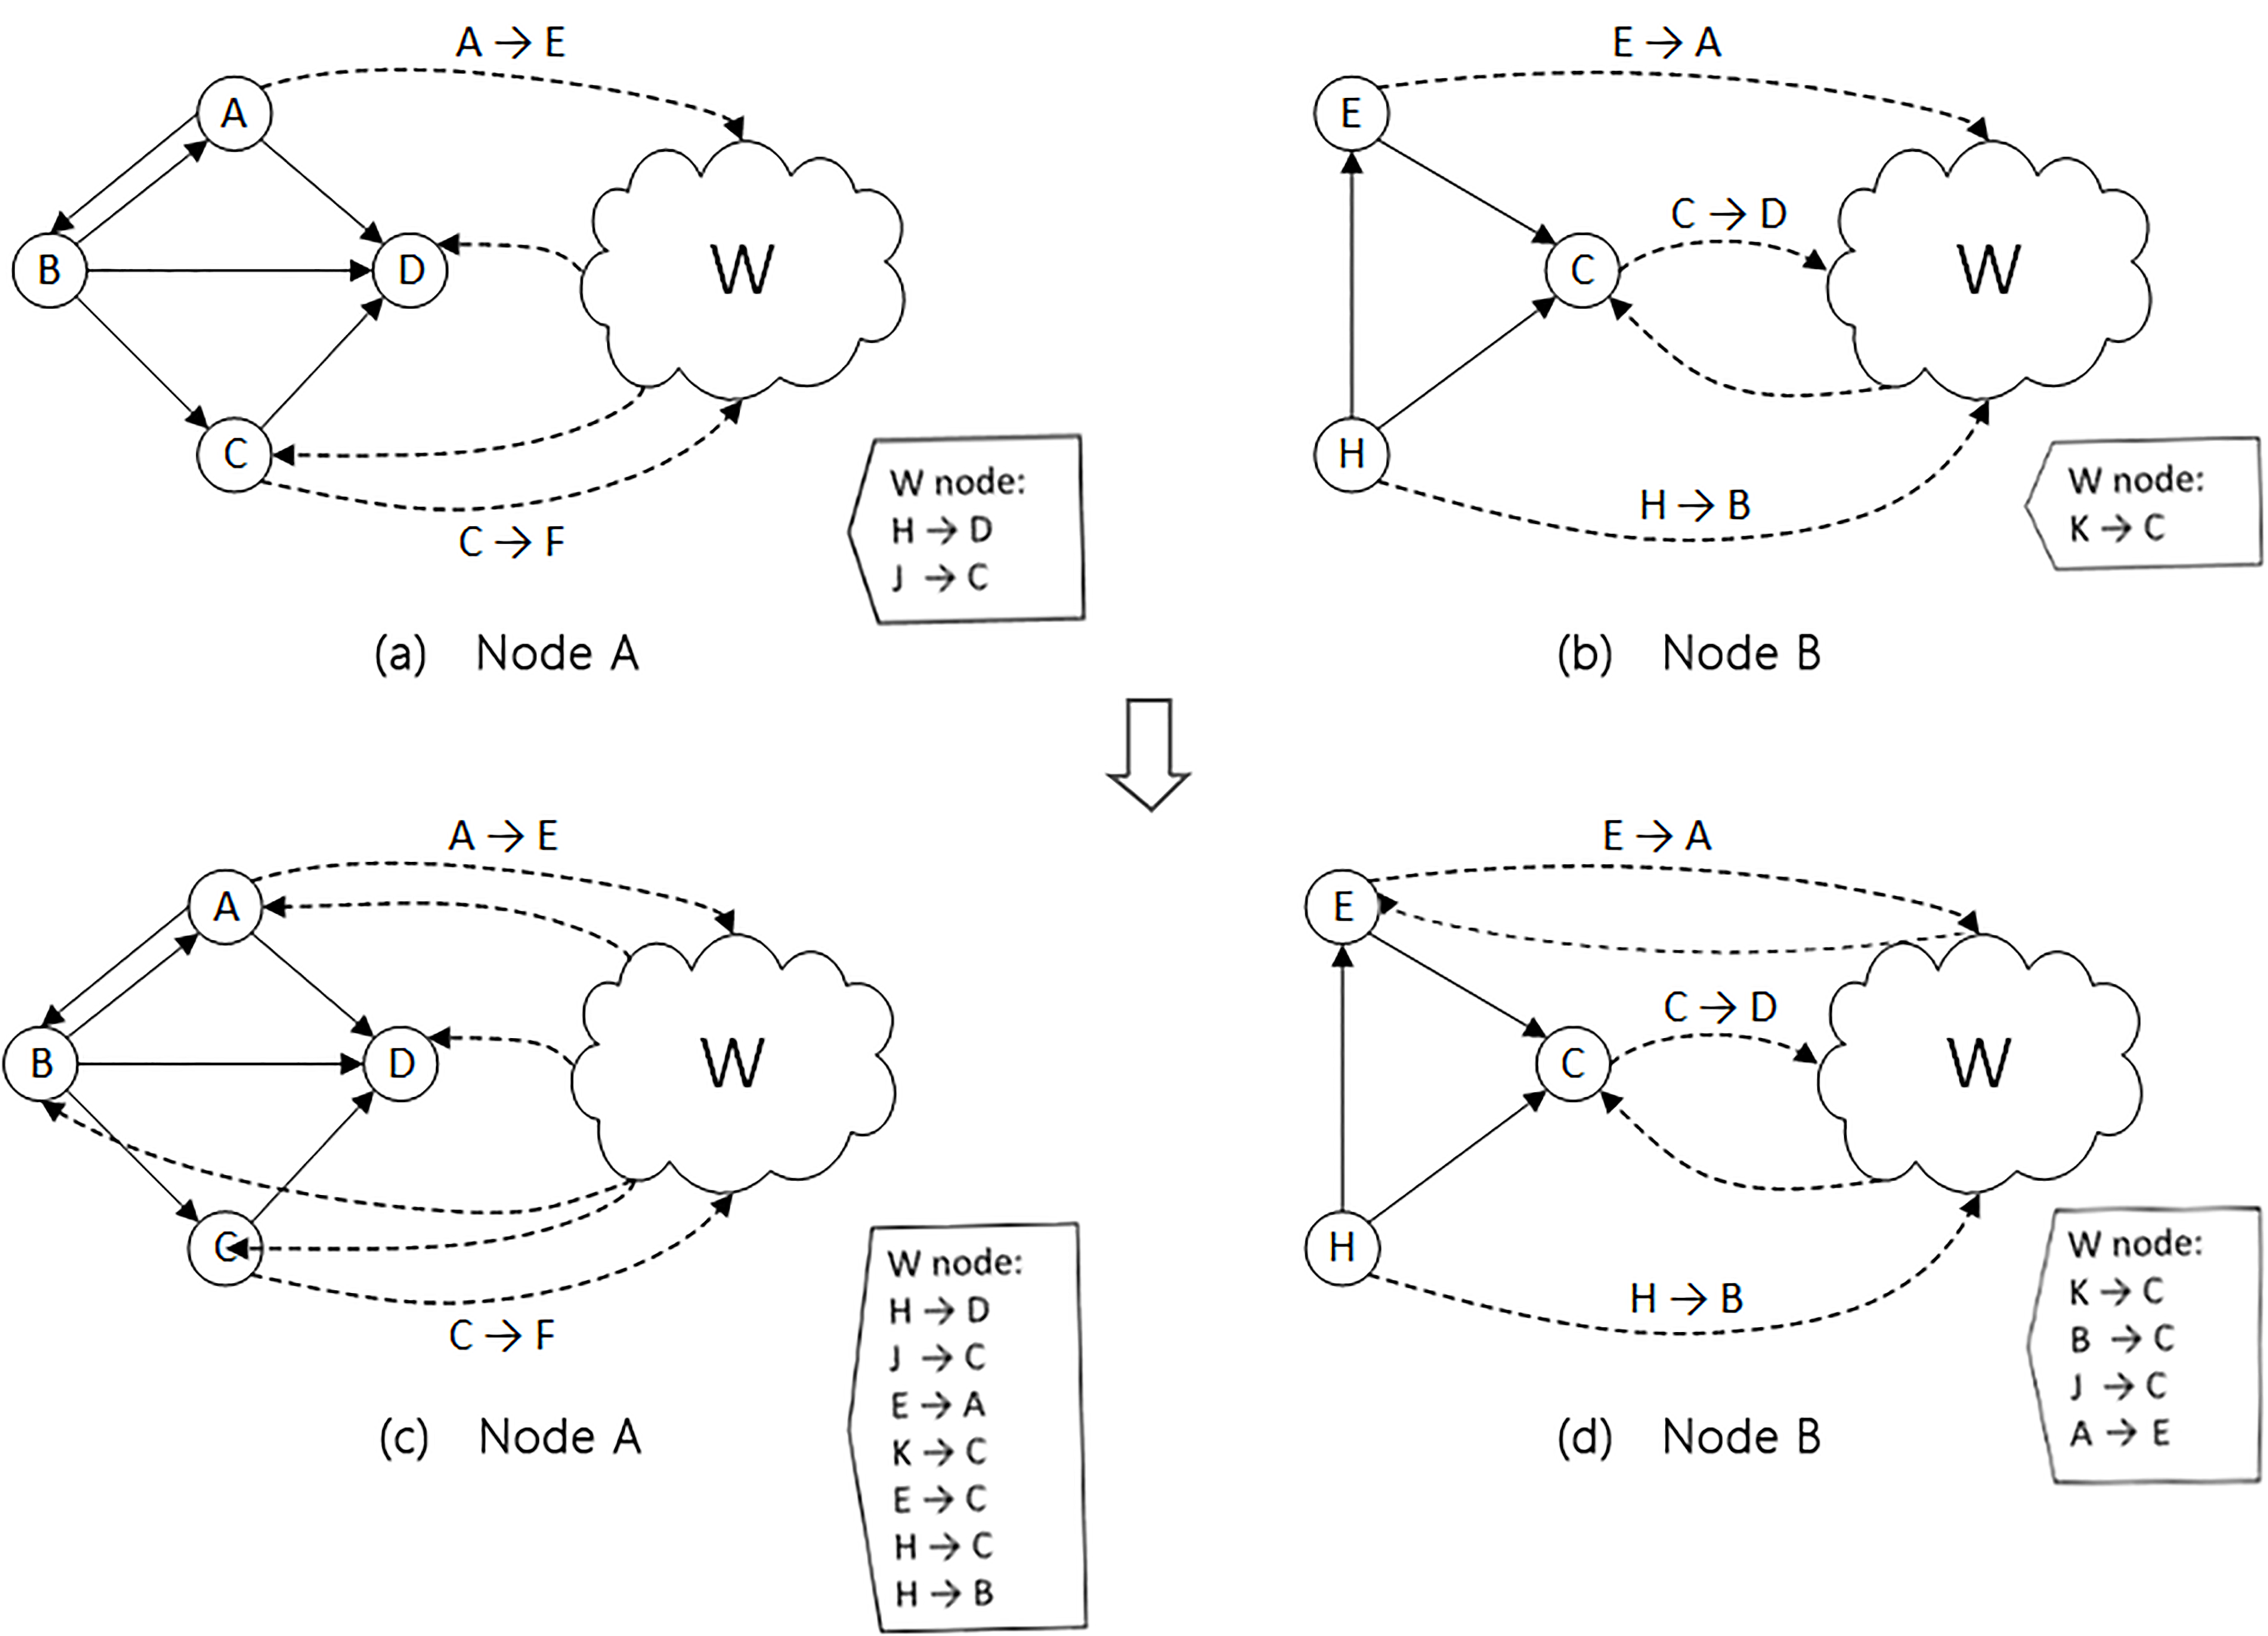
\includegraphics[scale=0.048]{imgs/Fig3.png}
\column{0.5\textwidth}
\begin{itemize}
\item Starting with the local graph $G$ of a node, the node first extends $G$ by adding a special node $W$, called world node, which represents all nodes in the network that do not belong to $G$.
\item Since it is not sufficient to estimate the global score by only knowing the local information, nodes improve their knowledge by meeting other nodes and exchanging information, namely the extended local graph and the score list.
\end{itemize}
\end{columns}
\end{frame}

\begin{frame}{3. Content Dissemination Model}
\framesubtitle{Decentralized Weighted PageRank-style Node Selection Algorithm - \textcolor{red}{Parameters Approximation}}
\begin{columns}
\column{0.5\textwidth}
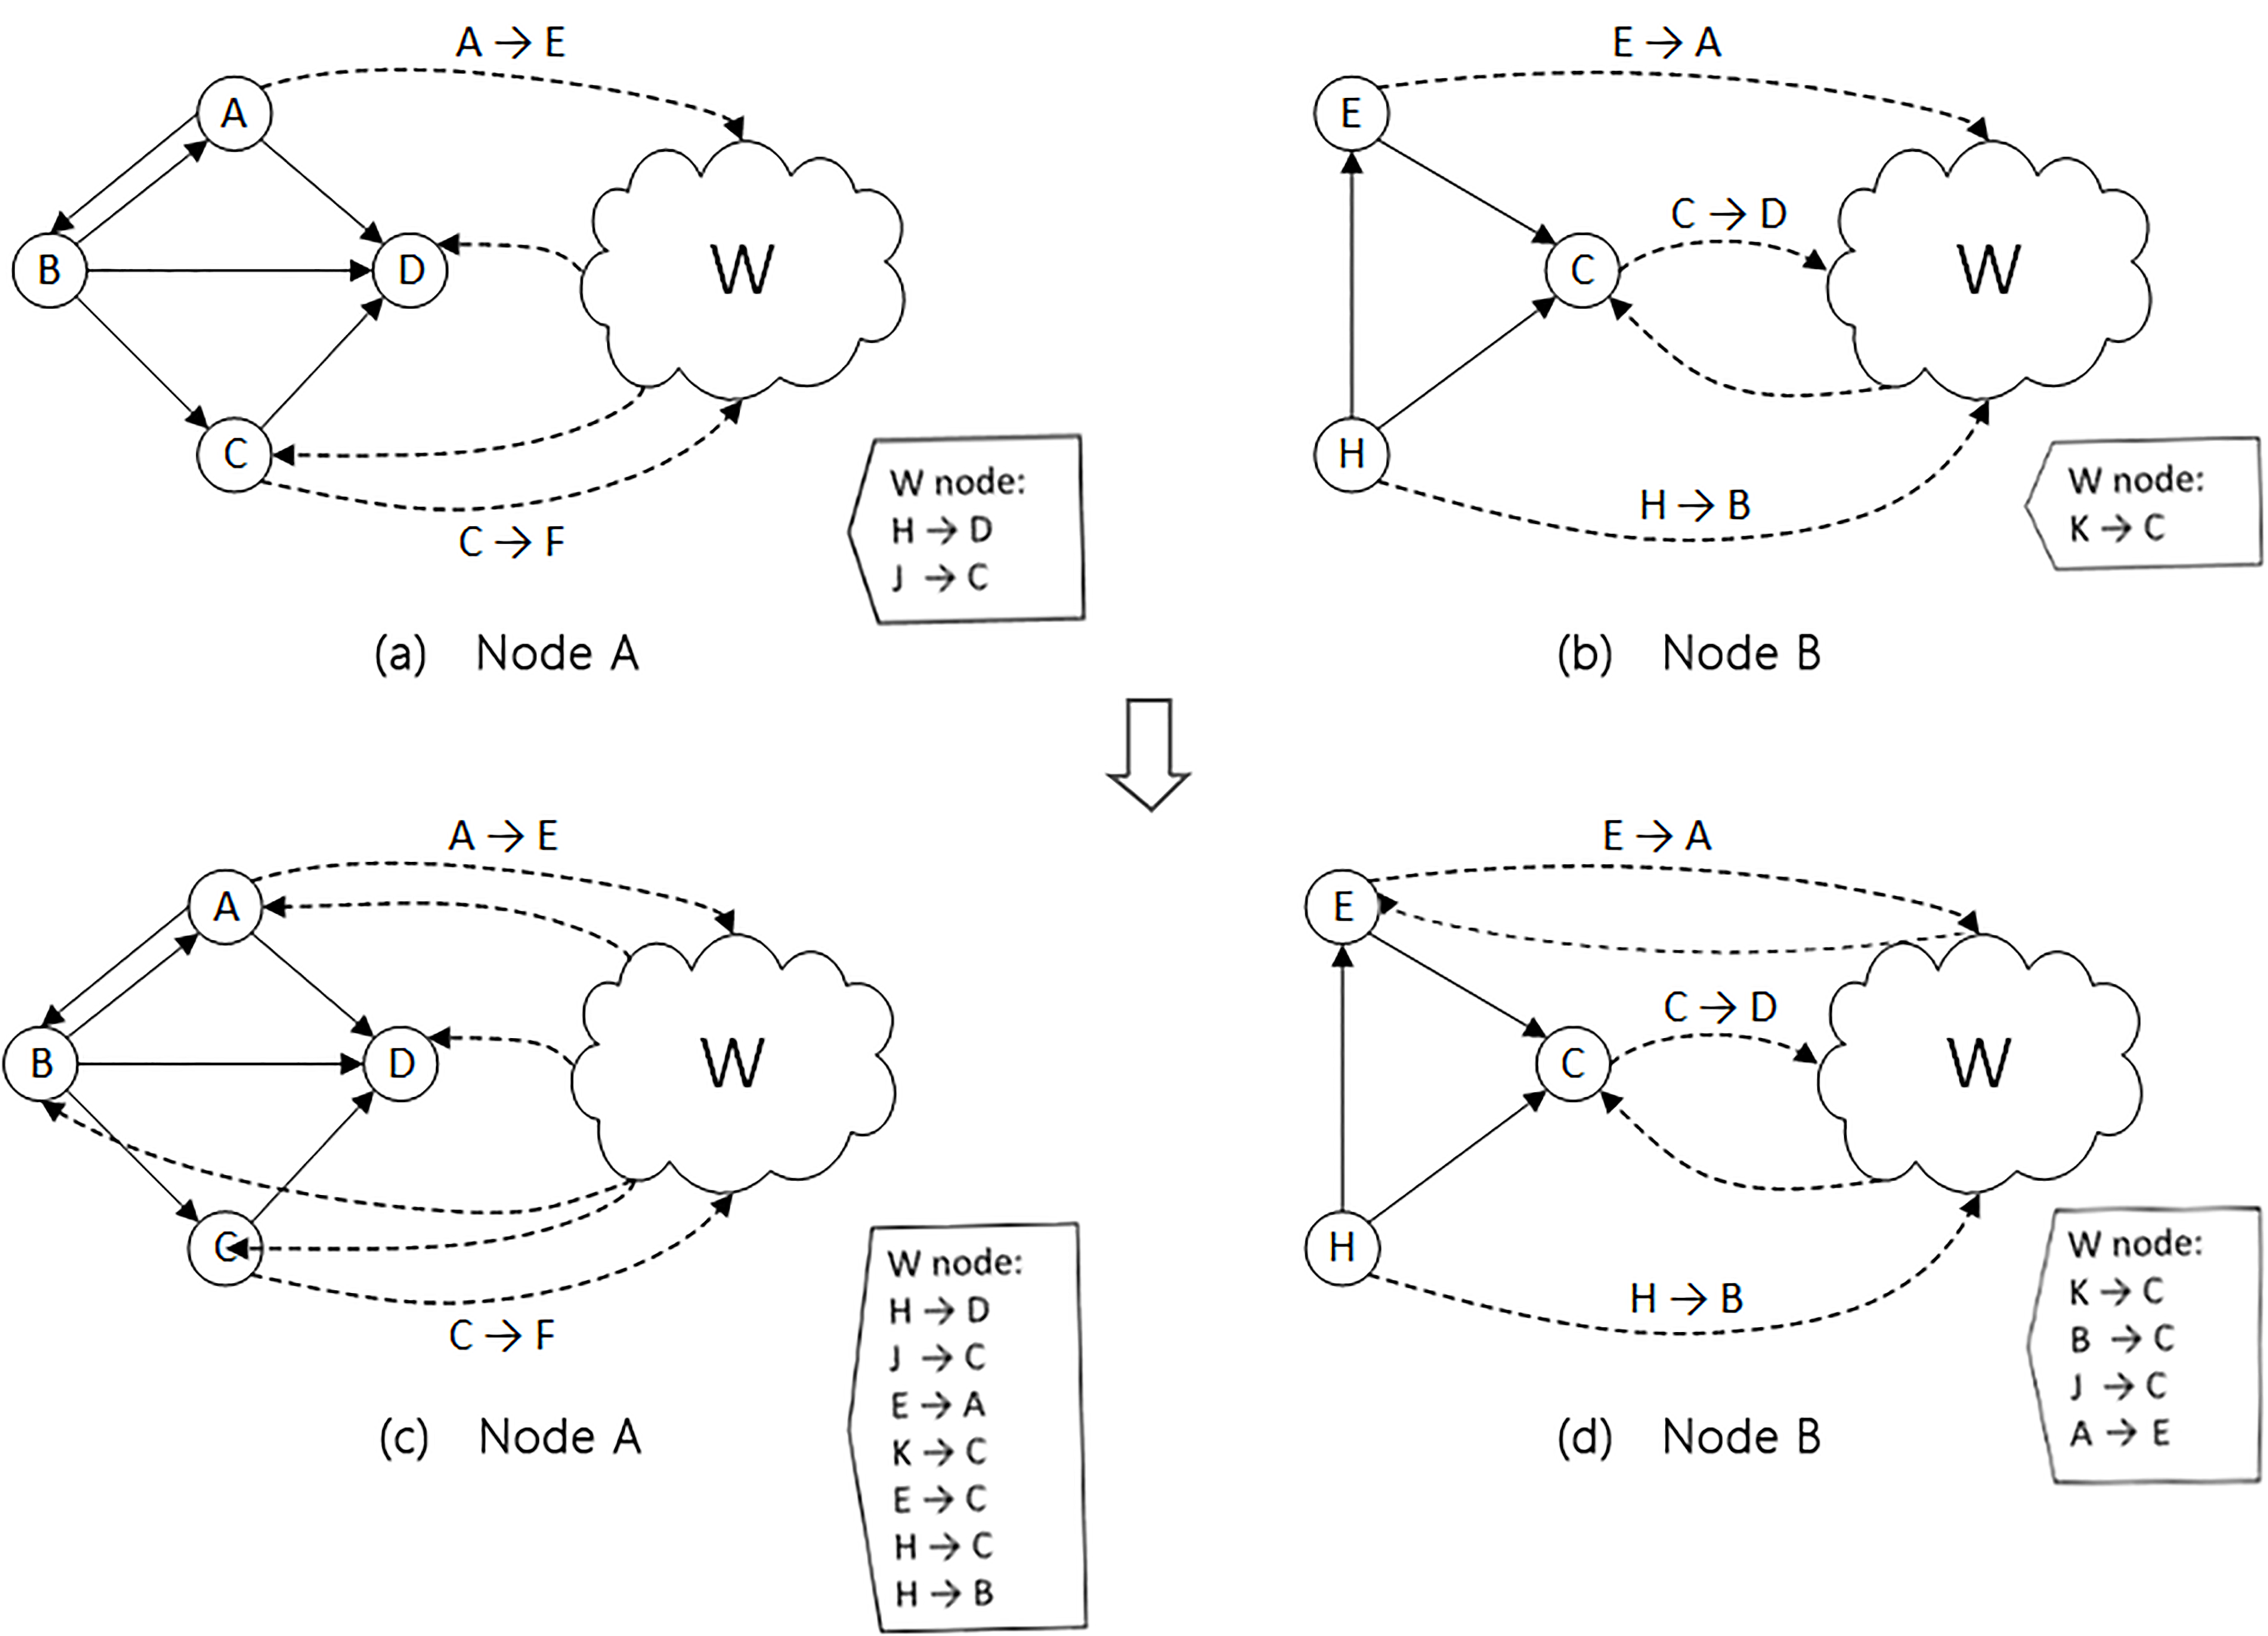
\includegraphics[scale=0.048]{imgs/Fig3.png}
\column{0.5\textwidth}
\begin{itemize}
    \item The graphs in figure (a) (b) represent the original local graphs of nodes A and B before their encounter. The graphs in figure (c) (d) represent the updated ones after the encounter. 
    \item A dashed arrow indicates that either start point or end point of the link is world node. Conversely, the meaning of a solid arrow is that both ends of the link are local nodes.
\end{itemize}
\end{columns}
\end{frame}

\begin{frame}{3. Content Dissemination Model}
\framesubtitle{Decentralized Weighted PageRank-style Node Selection Algorithm - \textcolor{red}{Parameters Approximation}}
\begin{columns}
\column{0.5\textwidth}
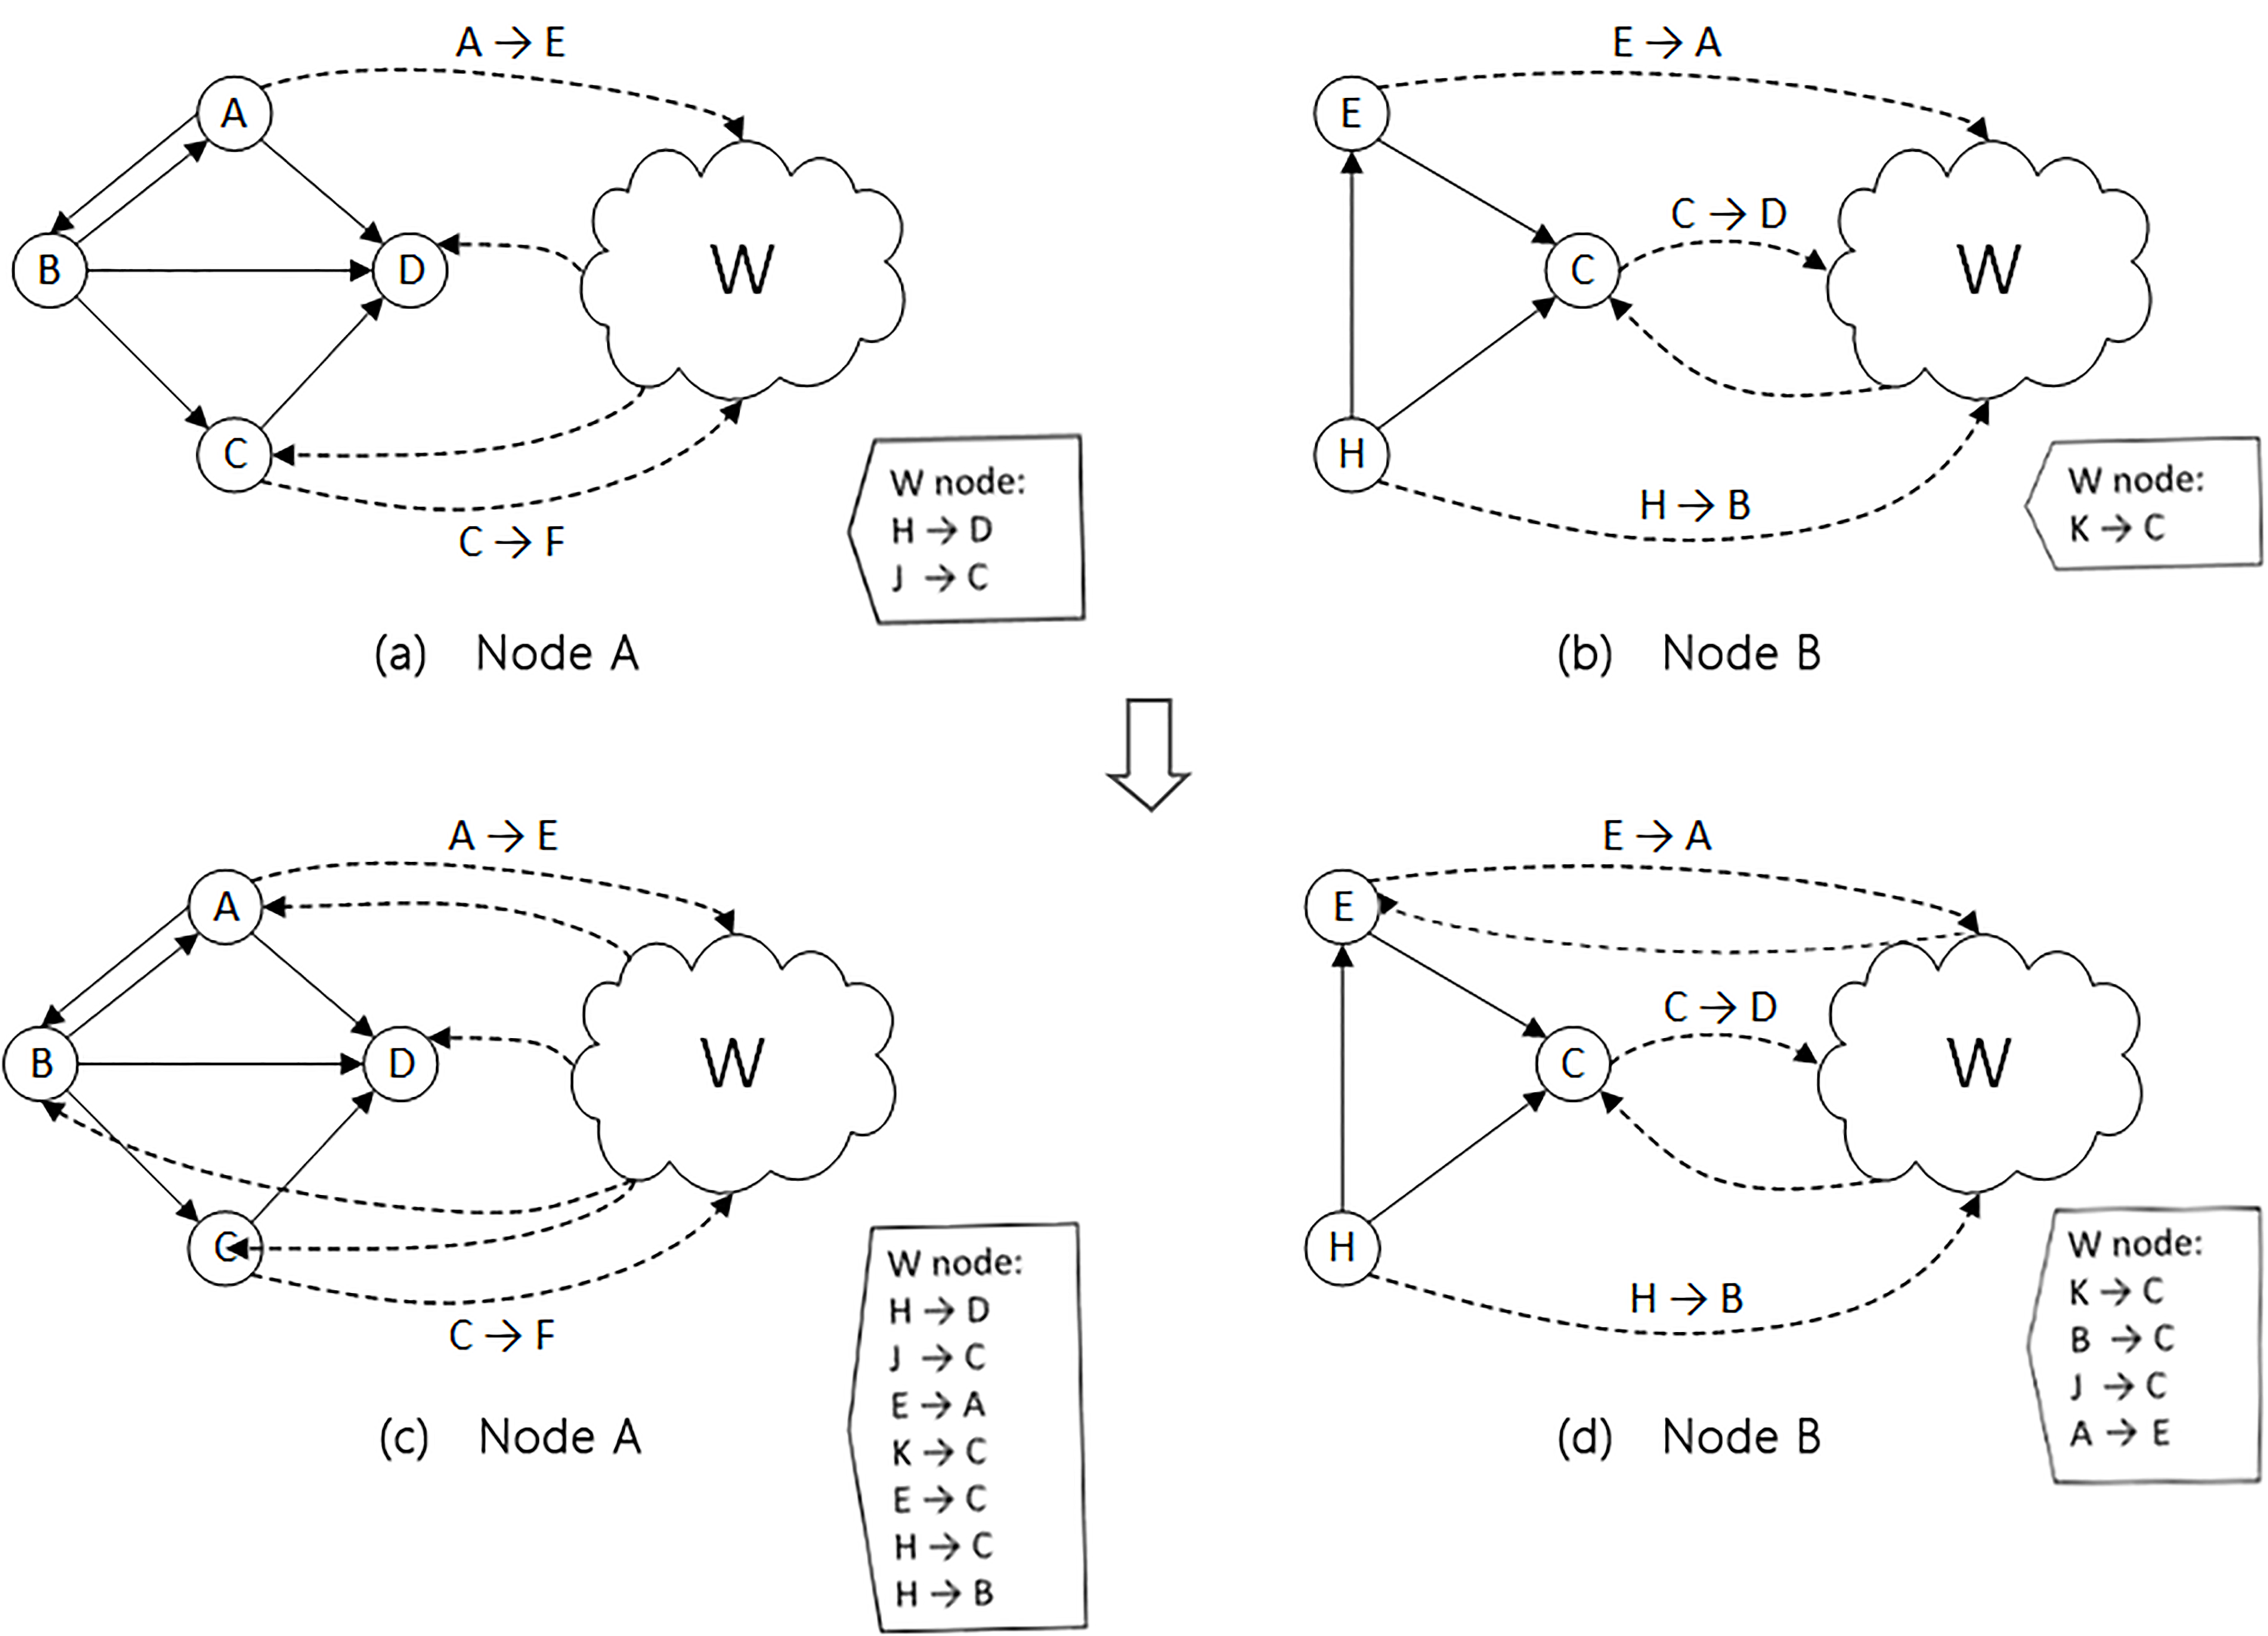
\includegraphics[scale=0.048]{imgs/Fig3.png}
\column{0.5\textwidth}
\begin{itemize}
    \item At a meeting, instead of merging the graphs and world nodes, only relevant information received from the other node into the local world node will be added. 
    \item The only changes are due to insertion of links from the world node to local nodes, whereas links from local nodes to the world node are invariant during all iterations.
\end{itemize}
\end{columns}
\end{frame}

\begin{frame}{3. Content Dissemination Model}
\framesubtitle{Decentralized Weighted PageRank-style Node Selection Algorithm - \textcolor{red}{Parameters Approximation}}
\begin{columns}
\column{0.5\textwidth}
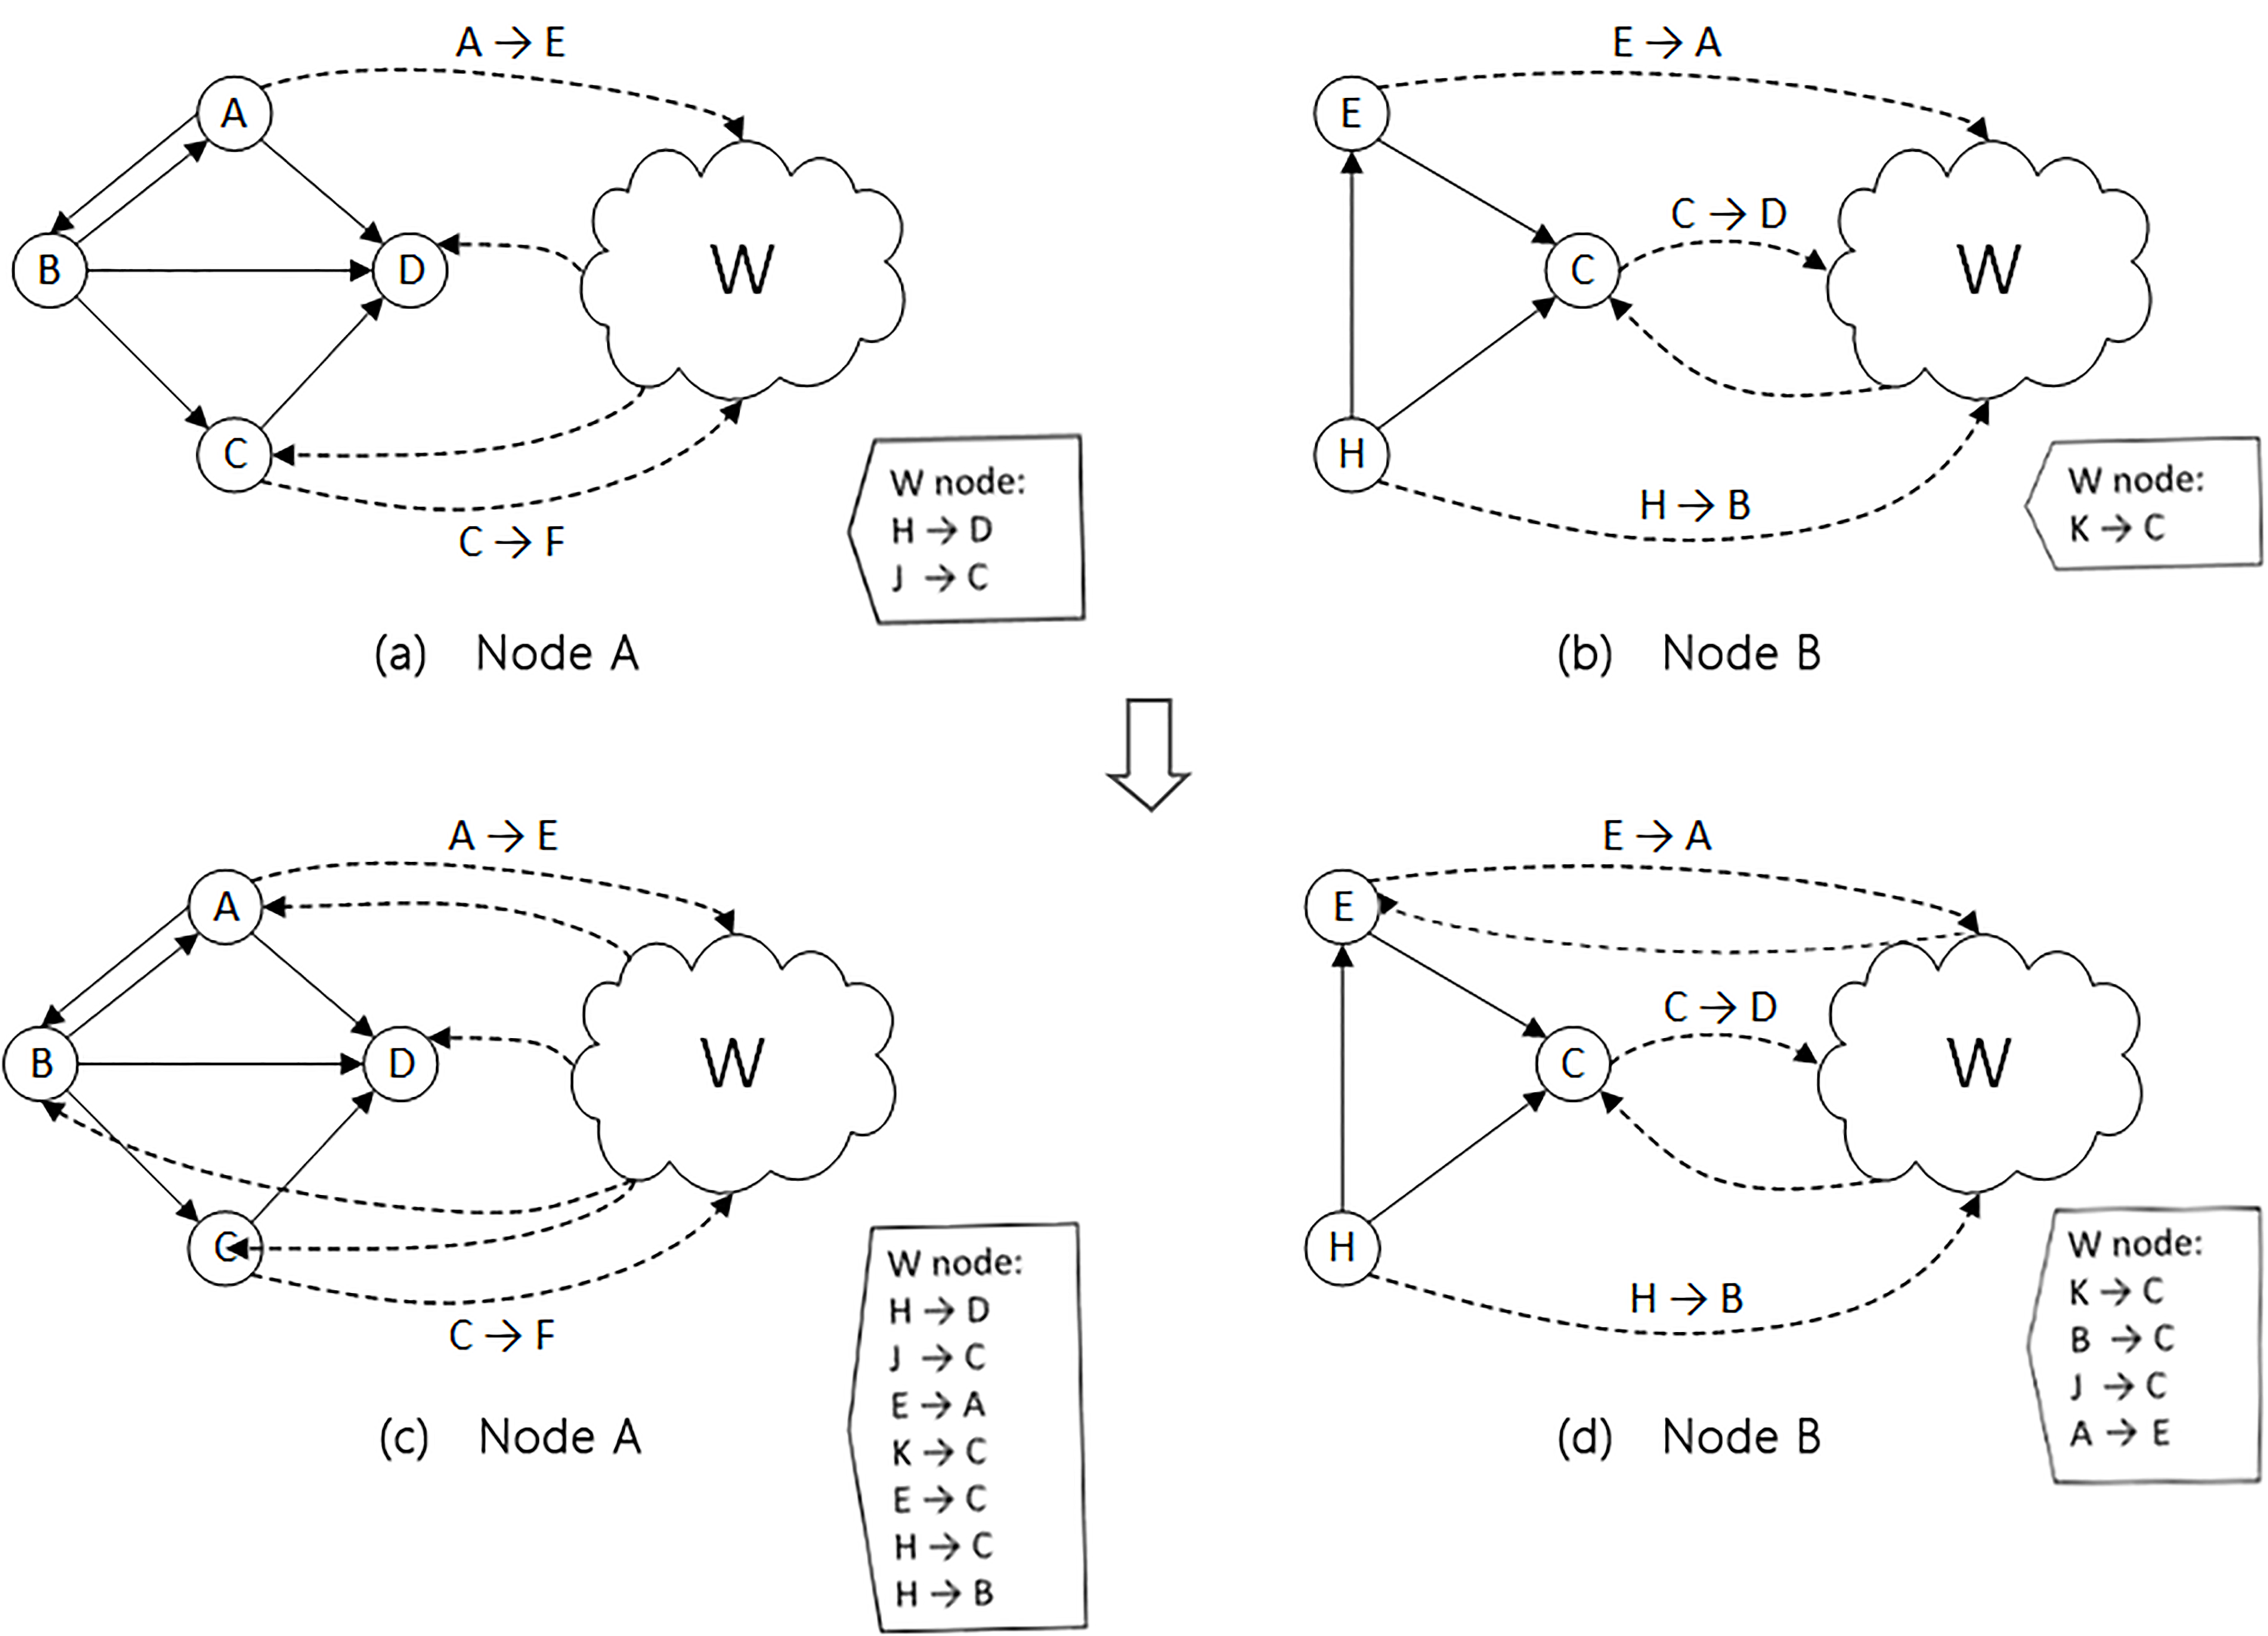
\includegraphics[scale=0.048]{imgs/Fig3.png}
\column{0.5\textwidth}
\begin{itemize}
    \item Firstly, updating node $A$. Obviously, we need to find links in node $B$ that points to the vertex in the vertex set of node $A$: 
    \begin{align*}
    &C\rightarrow D, E\rightarrow A, K\rightarrow C,\\
    &E\rightarrow C, H\rightarrow C, H\rightarrow B
    \end{align*}
    
    
    \item Since the link from $C$ to $D$ already exists in node $A$, it can be removed from the set. Then these links are added to the local graph of node $A$, as shown in figure (c).
\end{itemize}
\end{columns}
\end{frame}

\begin{frame}{3. Content Dissemination Model}
\framesubtitle{Decentralized Weighted PageRank-style Node Selection Algorithm - \textcolor{red}{Parameters Approximation}}
\begin{columns}
\column{0.5\textwidth}
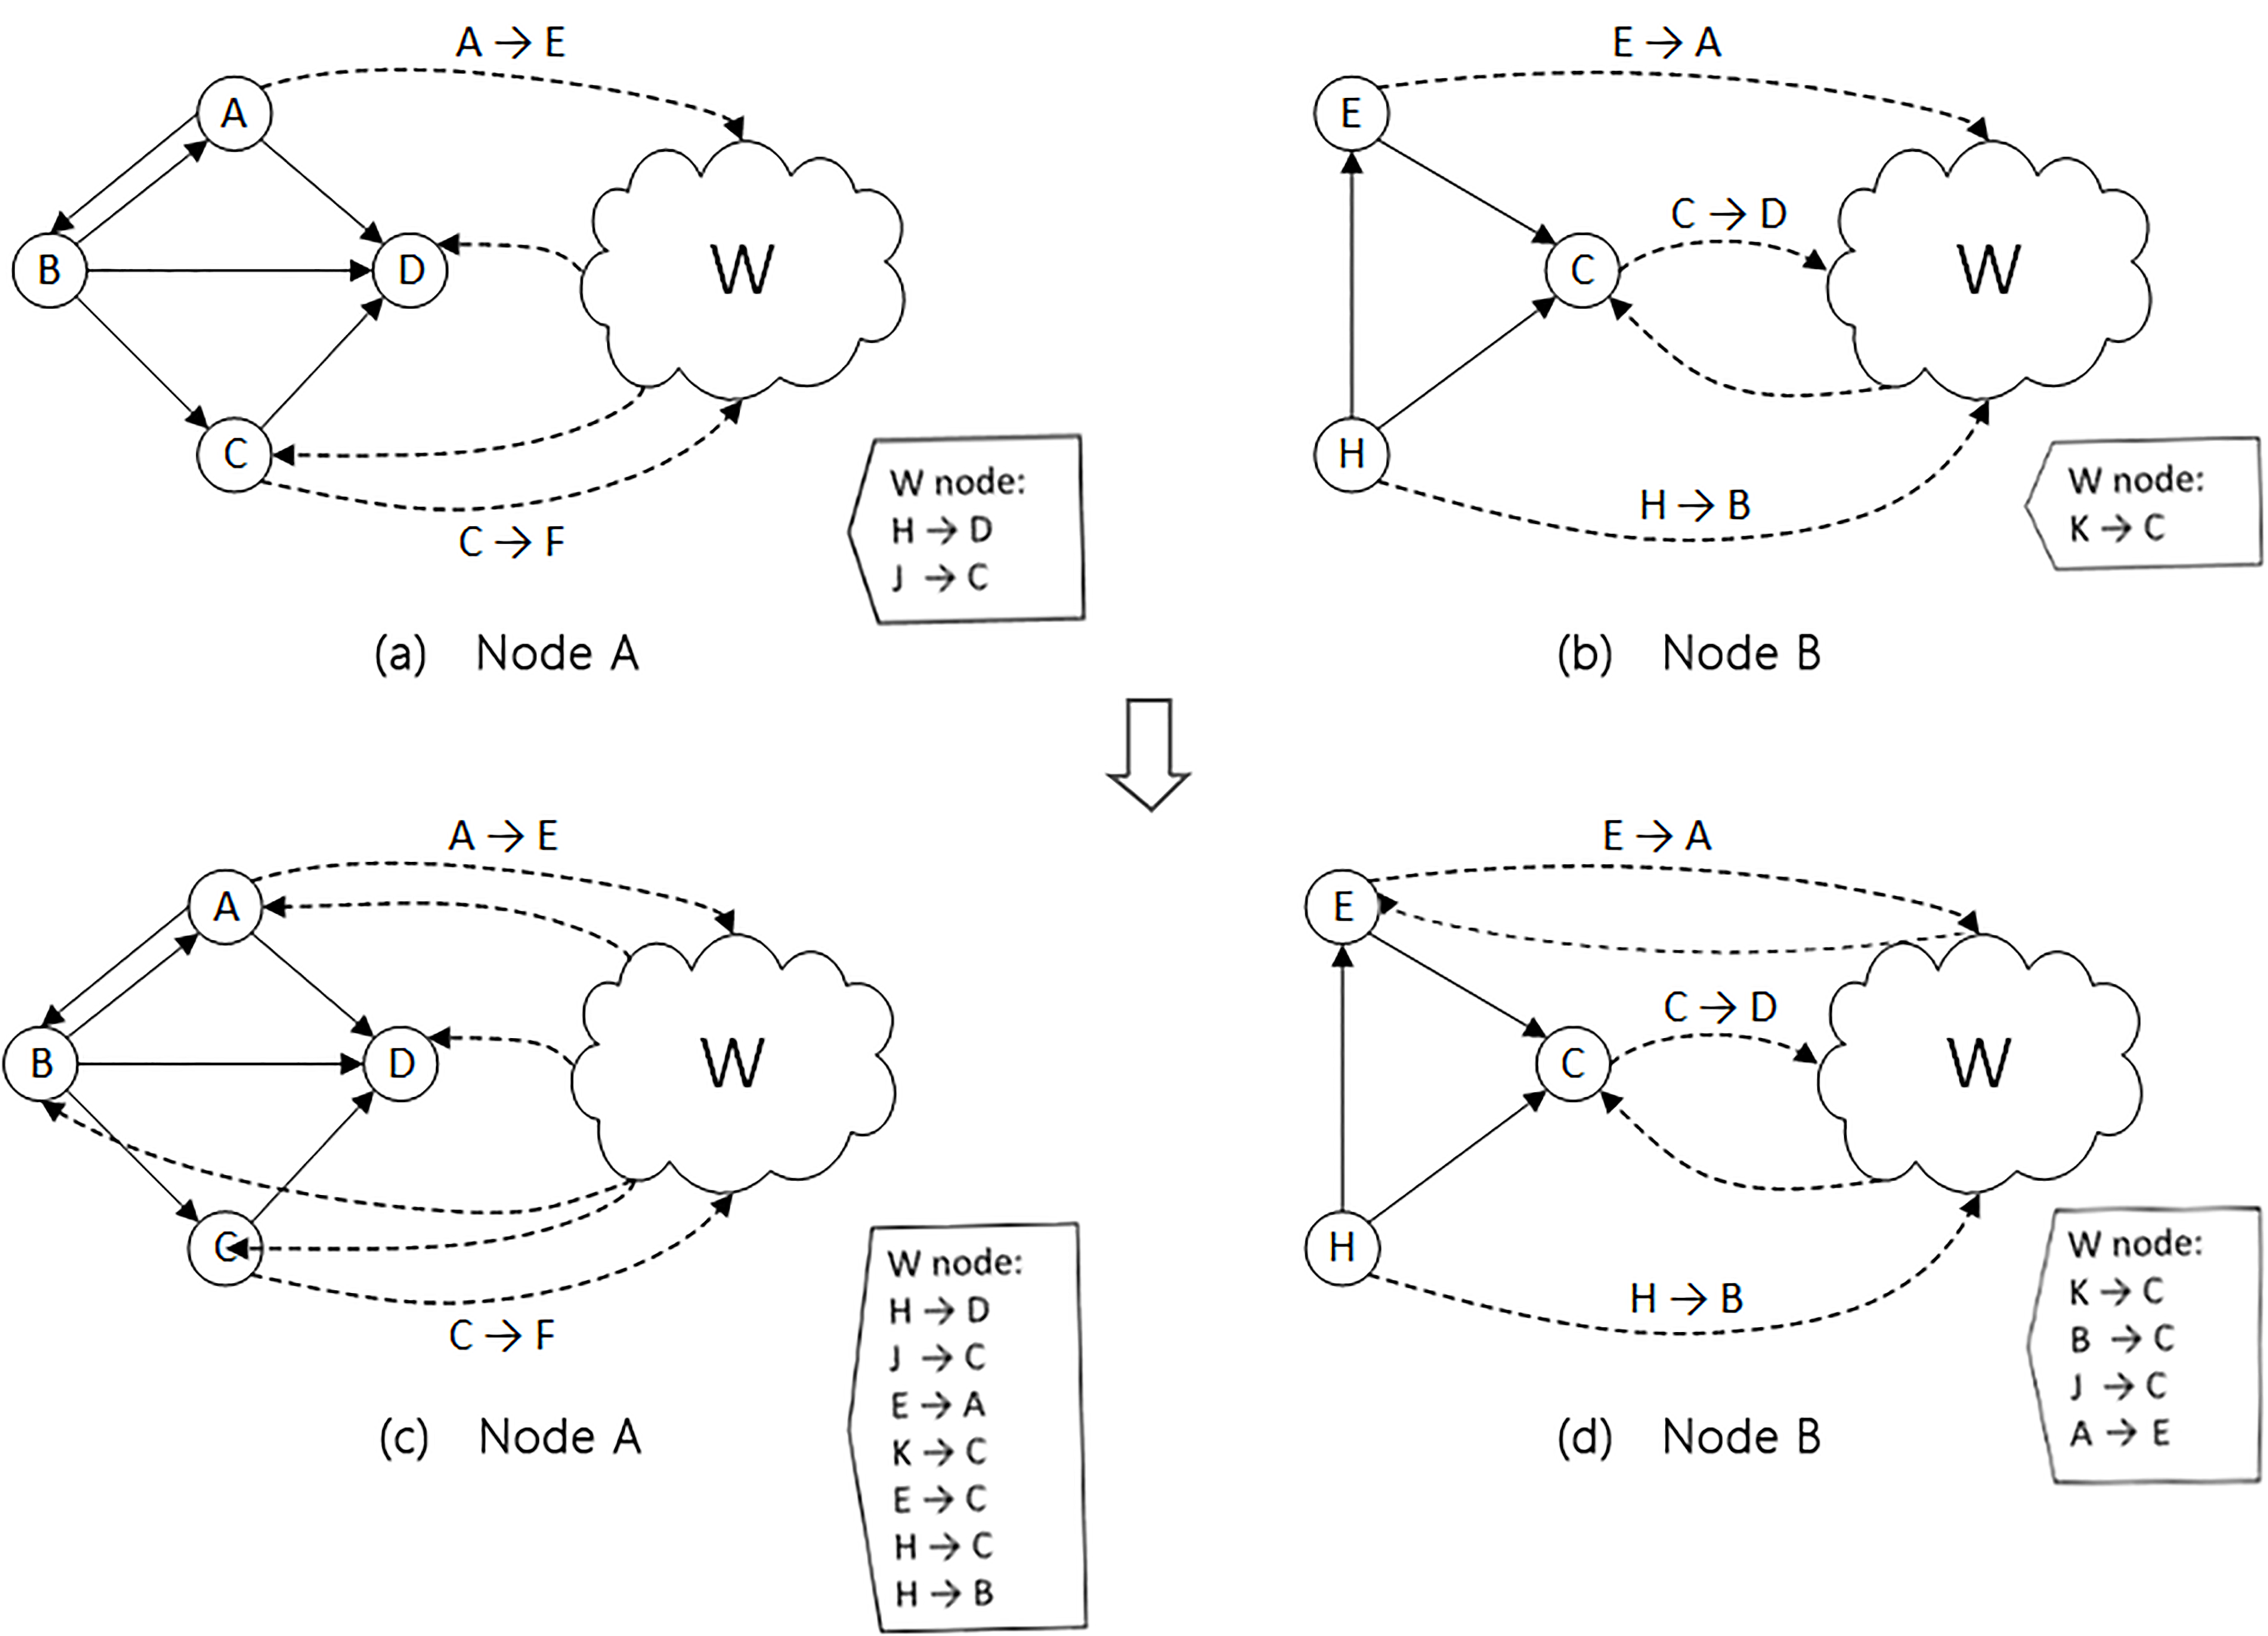
\includegraphics[scale=0.048]{imgs/Fig3.png}
\column{0.5\textwidth}
\begin{itemize}
   \item Secondly, updating node $B$. Similarly, we need to find links in node $A$ that points to the vertex in the vertex set of node $B$: \[{B\rightarrow C,J\rightarrow C,A\rightarrow E}\] Then these links are added to the local graph of node $B$. The updated node $B$ is shown in figure 3(d).
\end{itemize}
\end{columns}
\end{frame}



\begin{frame}{Outline}
\begin{enumerate}[1. ]
\uncover<>{\item Introduction}
\uncover<>{\item Related Works}
\uncover<>{\item Content Dissemination Model}
\uncover<1>{\item Evaluation}
\uncover<>{\item Future Work}
\uncover<>{\item Conclusion}
\end{enumerate}
\end{frame}



\begin{frame}{4. Evaluation}
\begin{itemize}
    \item \textbf{Experimental Setup}
    \item \textbf{Baseline Algorithms for Comparison}
    \begin{itemize}
        \item Maximum degree method
        \item EasyRank method
    \end{itemize}
    \item \textbf{Metrics}
    \begin{itemize}
        \item The number of nodes that meet the required coverage requirement
        \item The distribution makespan
        \item The mean of coverage
        \item The average latency
    \end{itemize}
    \item \textbf{Result Analysis}
    \item \textbf{Discussion}
\end{itemize}
\end{frame}

\begin{frame}{4. Evaluation}
\framesubtitle{Experimental Setup}
\centering
\begin{table}[]
    \centering
    \newcolumntype{Y}{>{\centering\arraybackslash}X}
    \begin{tabularx}{\textwidth}{c|c|Y}
    \Xhline{1.5pt}
     \textbf{Symbol} & \textbf{Hyper-parameters} & \textbf{Value} \\
     \hline \hline
     $Q$ & The number of quotas & Ten percent of the total number of nodes \\
     \hline
     $F$ & File size & 1MB \\
     \hline
     $C$ & Coverage requirement & $0.1$\\
     \hline
     $B$ & Bandwidth allocation & 640kbps: 40\%, 1Mbps: 40\%, 2Mbps: 10\%, 4Mbps: 10\% \\
     \hline
     $m$ & The number of interactions & Ten percent of the total number of nodes \\
     \hline
     $E$ & The number of edge servers & 5\\
\Xhline{1.5pt}     
\end{tabularx}
\caption{Simulation Hyper-parameters}
\end{table}
\end{frame}


\begin{frame}{4. Evaluation}
\framesubtitle{Baseline Algorithms for Comparison}
In our decentralized PageRank-based content dissemination model, the node selection algorithm is the core of the model. Therefore, different node selection algorithms are compared here. 
\begin{itemize}
    \item \textbf{Maximum degree method}
    \begin{itemize}
        \item Generally, nodes with more connections are considered more important. 
        \item However, to some extent, the degree can only reflect the direct neighbor connections. It is inadequate for discovering the overall topology, such as how neighbors are connected with others in the network.
    \end{itemize}
    \item \textbf{EasyRank method}
    \begin{itemize}
        \item The EasyRank (\textit{Khan, M. A., Debnath, H., \& Borcea, C., 2016}) centrality is a function of the number of friends of its 1-hop neighbors.
        \item It assigns relatively higher scores to peers whose neighbors have few friends in order to reduce the skewness in storage availability and improve replication fairness/success.
    \end{itemize}
\end{itemize}
\end{frame}

\begin{frame}{4. Evaluation}
\framesubtitle{Metrics}
\begin{block}{The number of nodes that meet the required coverage requirement}
As the name suggests, this is a quantitative measurement.
\end{block}
\begin{block}{The distribution makespan}
It refers to the time spent by the entire model to complete the content dissemination process.
\end{block}
\begin{block}{The mean of coverage}
It means the average coverage of all nodes when the dissemination process finishes.
\end{block}
\begin{block}{The average latency}
It means the average latency of users accessing content.
\end{block}
\end{frame}

\begin{frame}{4. Evaluation}
\framesubtitle{Result Analysis}
\begin{columns}
\column{0.5\textwidth}
\begin{figure}
    \centering
    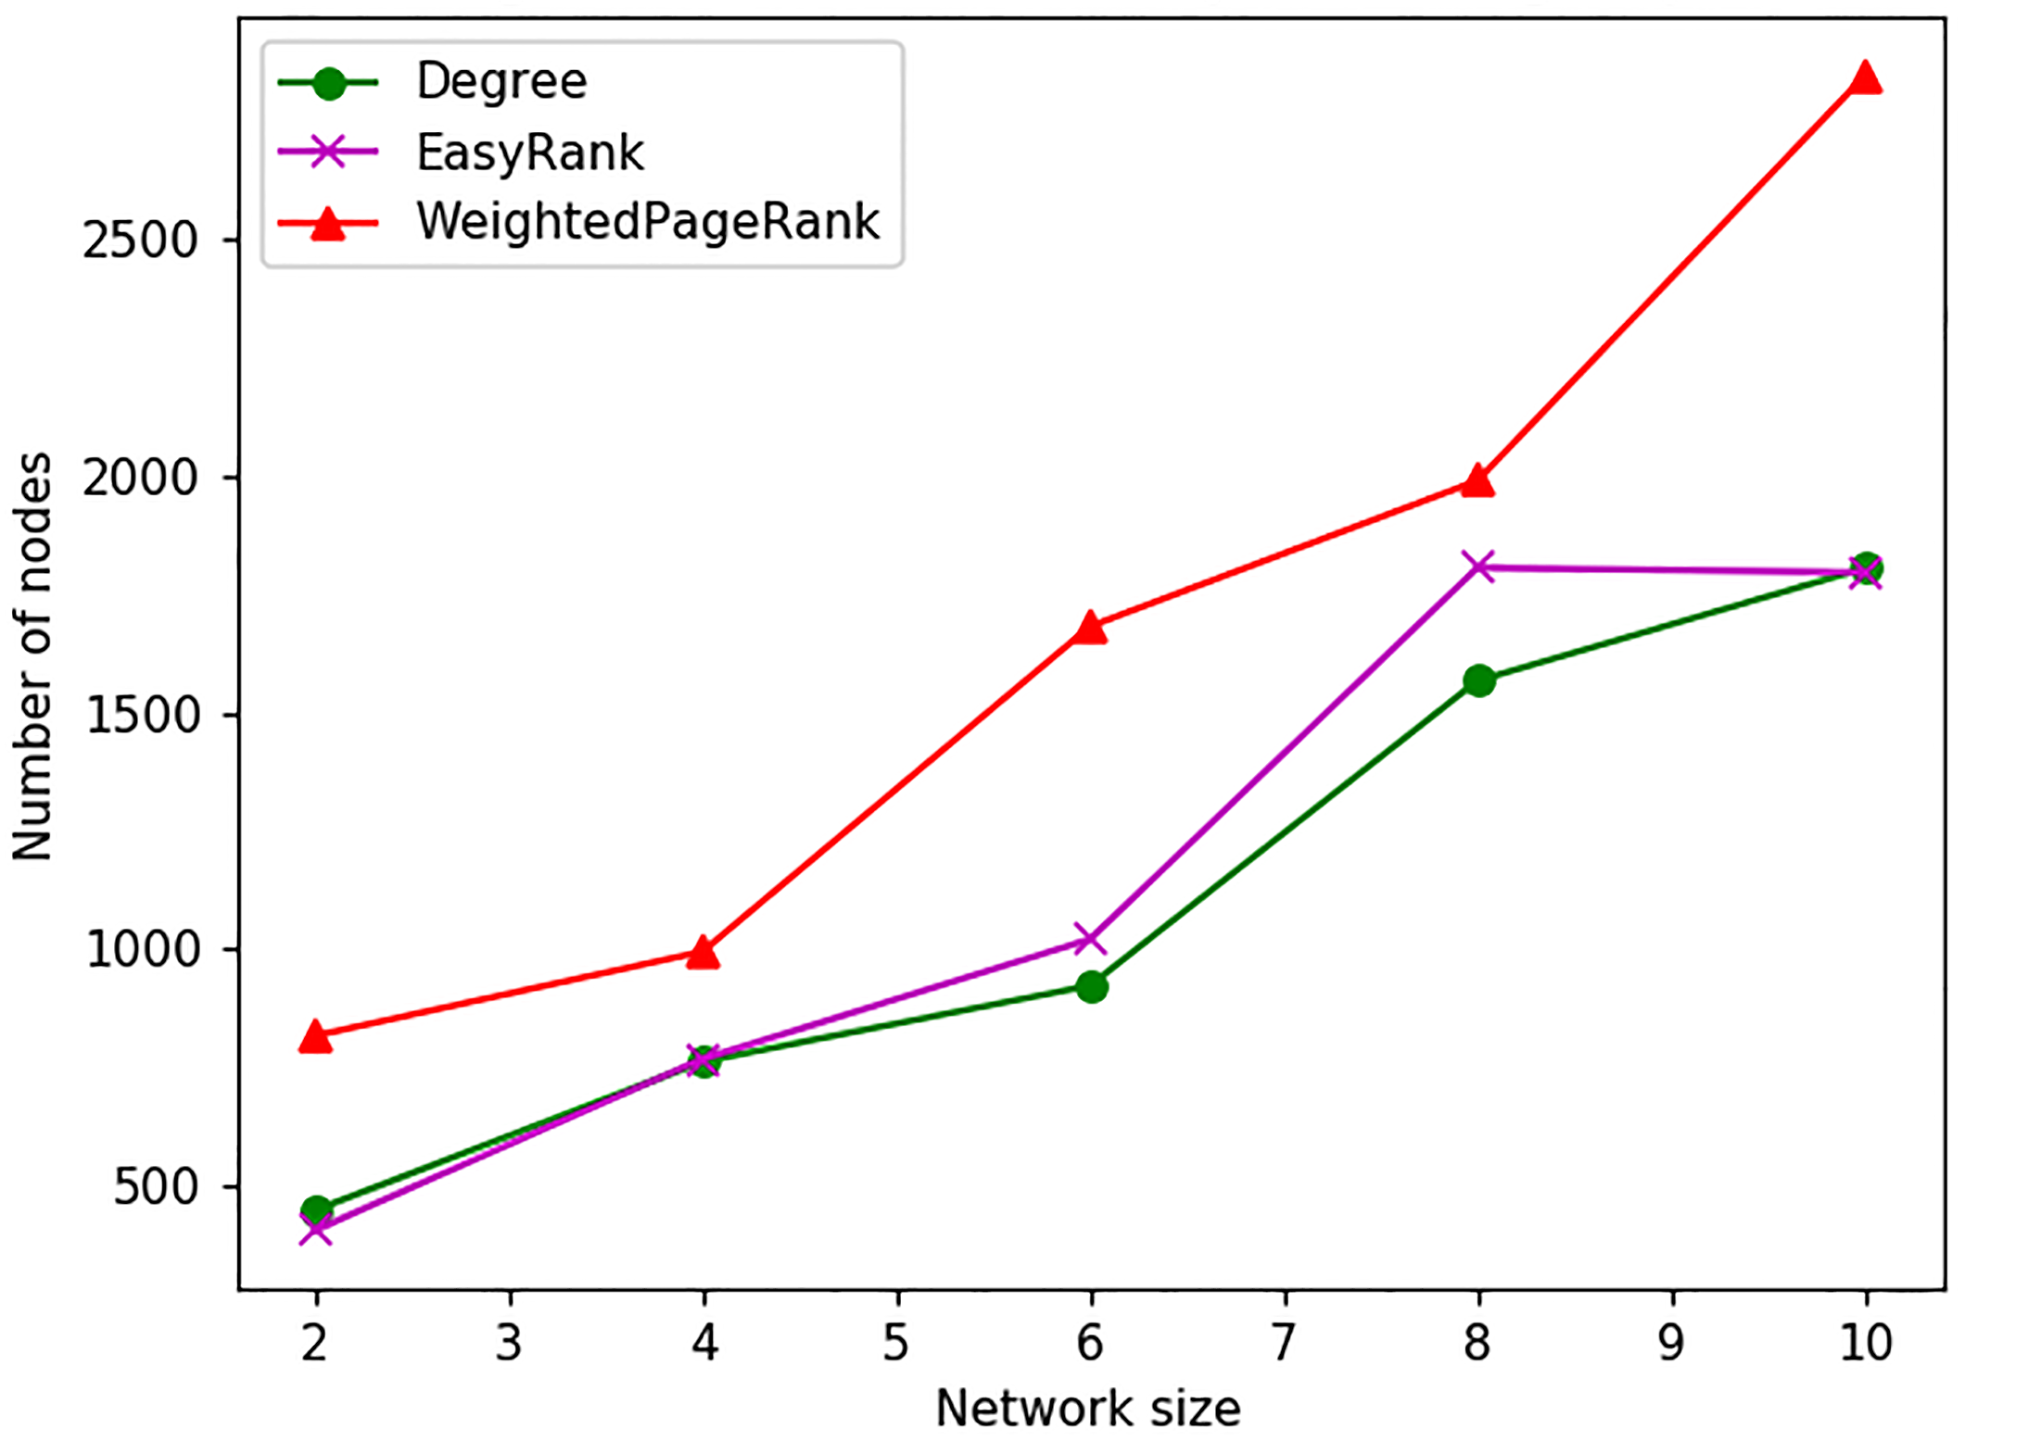
\includegraphics[width=0.9\textwidth]{imgs/Figure4.png}
    \caption{The percentage of nodes that meet the required coverage requirement}
\end{figure}
\column{0.5\textwidth}
Since the decentralized PageRank approximation introduces a certain degree of randomness, the ranking of neighbor nodes may be slightly different from that of the global PageRank. Therefore, not only nodes selected by the other two methods, but also the remaining nodes, are likely to be selected. While in degree and EasyRank method, replicas are just placed on nodes with more neighbors, which causes uneven distribution of the content.
\end{columns}
\end{frame}

\begin{frame}{4. Evaluation}
\framesubtitle{Result Analysis}
\begin{columns}
\column{0.5\textwidth}
\begin{figure}
    \centering
    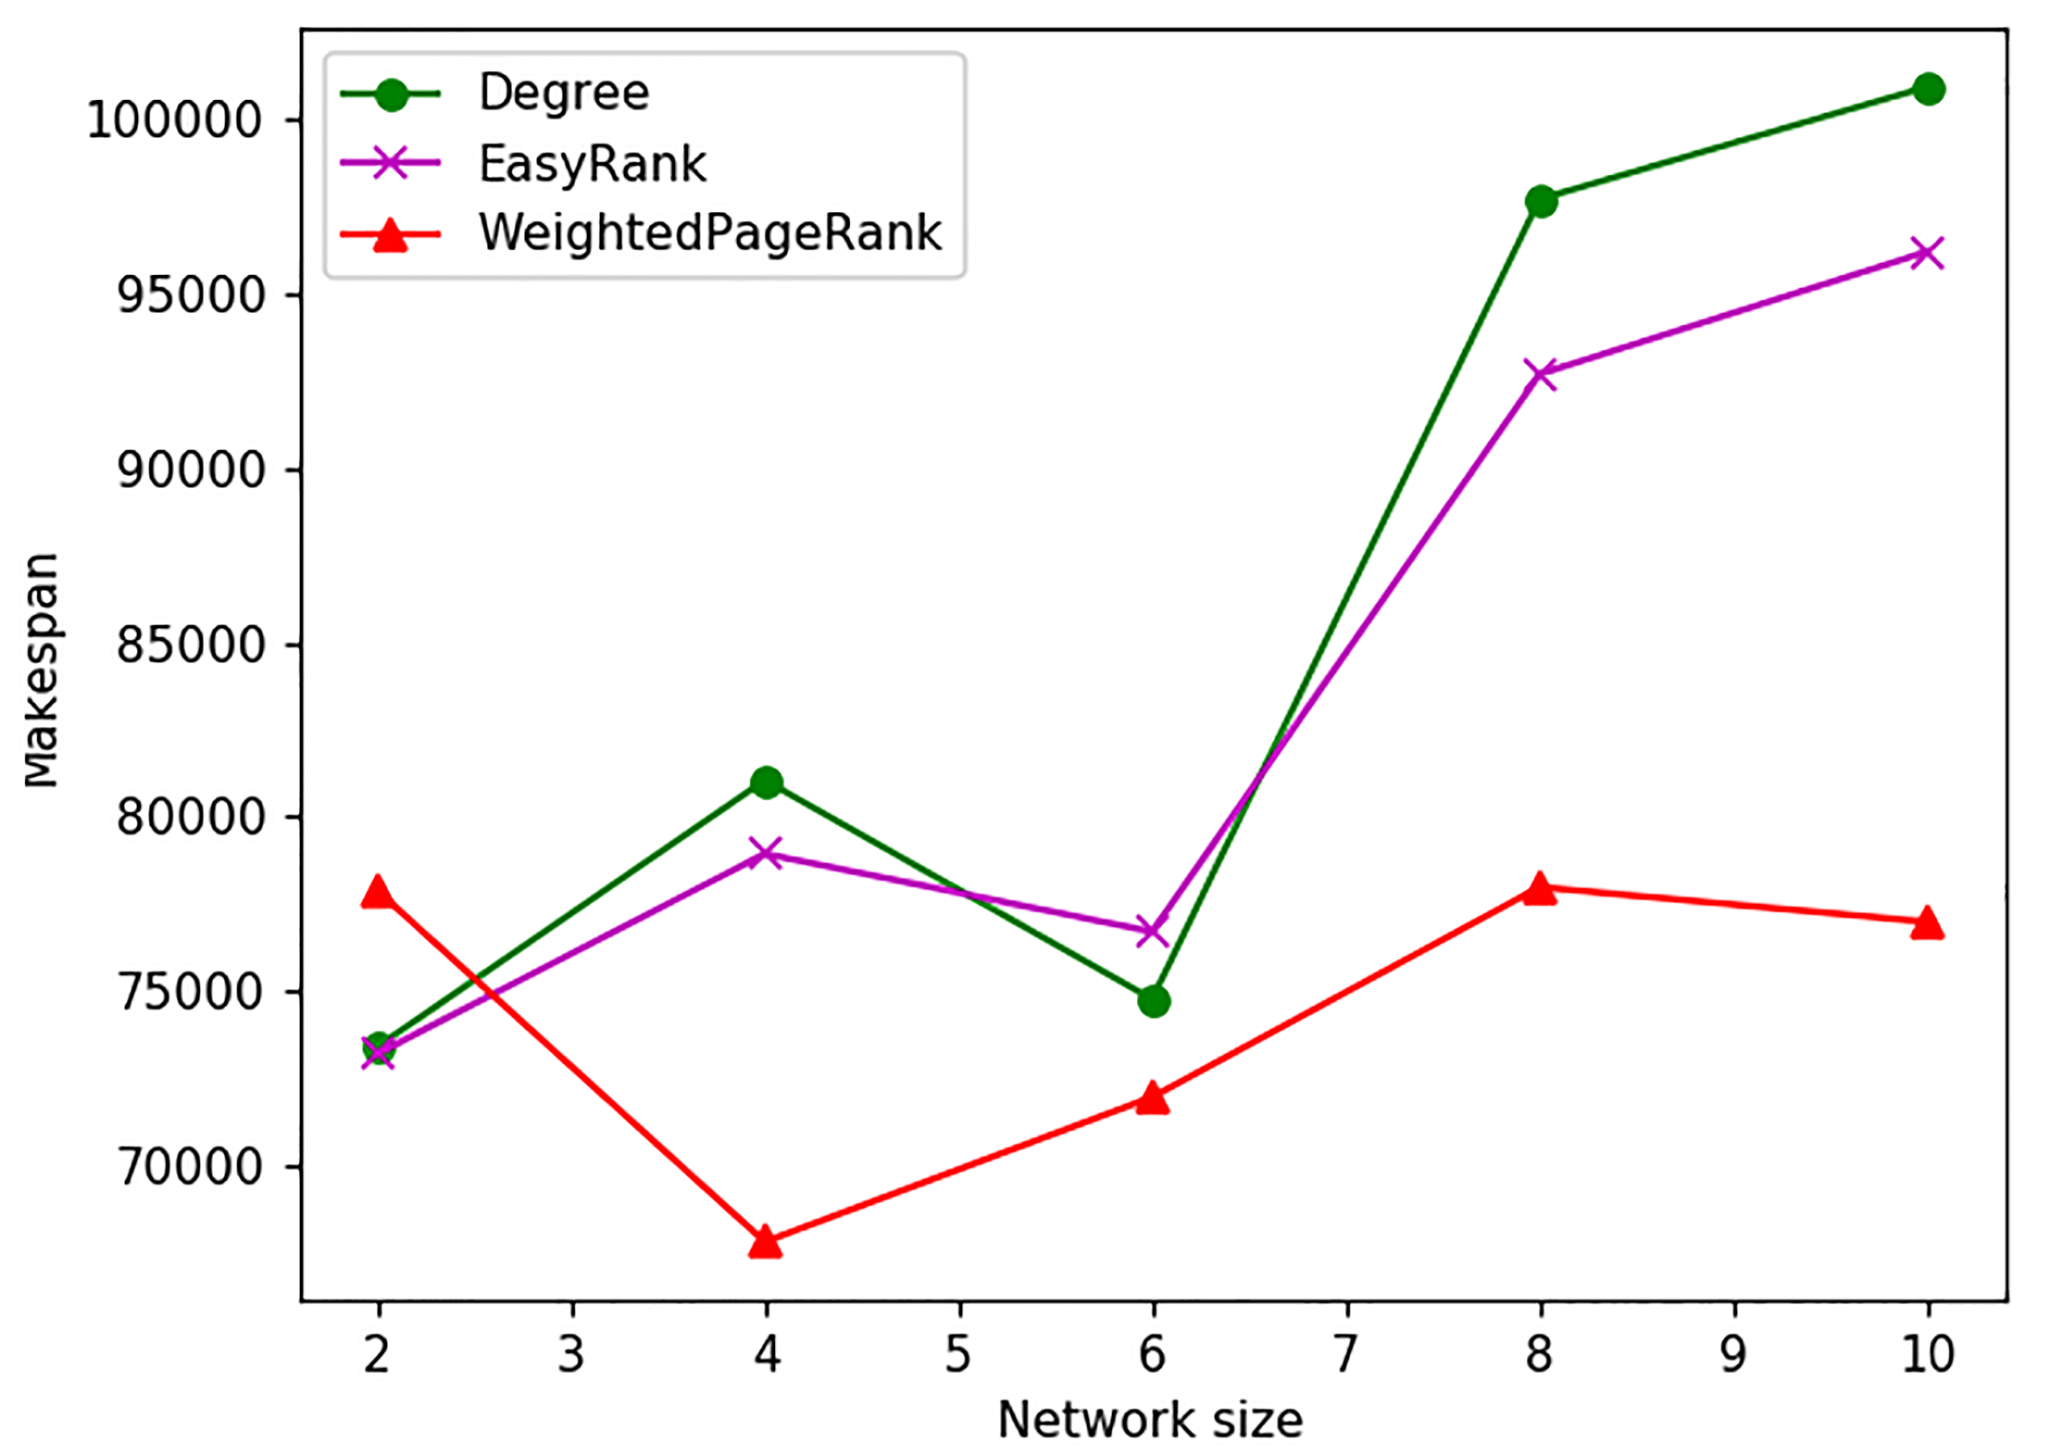
\includegraphics[width=0.9\textwidth]{imgs/Figure5.png}
    \caption{The dissemination makespan}
\end{figure}
\column{0.5\textwidth}
It can be seen that when the network size is 2000, the makespan of weighted PageRank is slightly higher than the other two methods, but as the network size increases, the makespan of weighted PageRank becomes significantly less than the maximum degree and the EasyRank method. This is because the weighted PageRank method incorporates the bandwidth as a significant part into the link weights between node links, while both the maximum degree and the EasyRank methods are not optimized for the bandwidth.
\end{columns}
\end{frame}

\begin{frame}{4. Evaluation}
\framesubtitle{Result Analysis}
\begin{columns}
\column{0.5\textwidth}
\begin{figure}
    \centering
    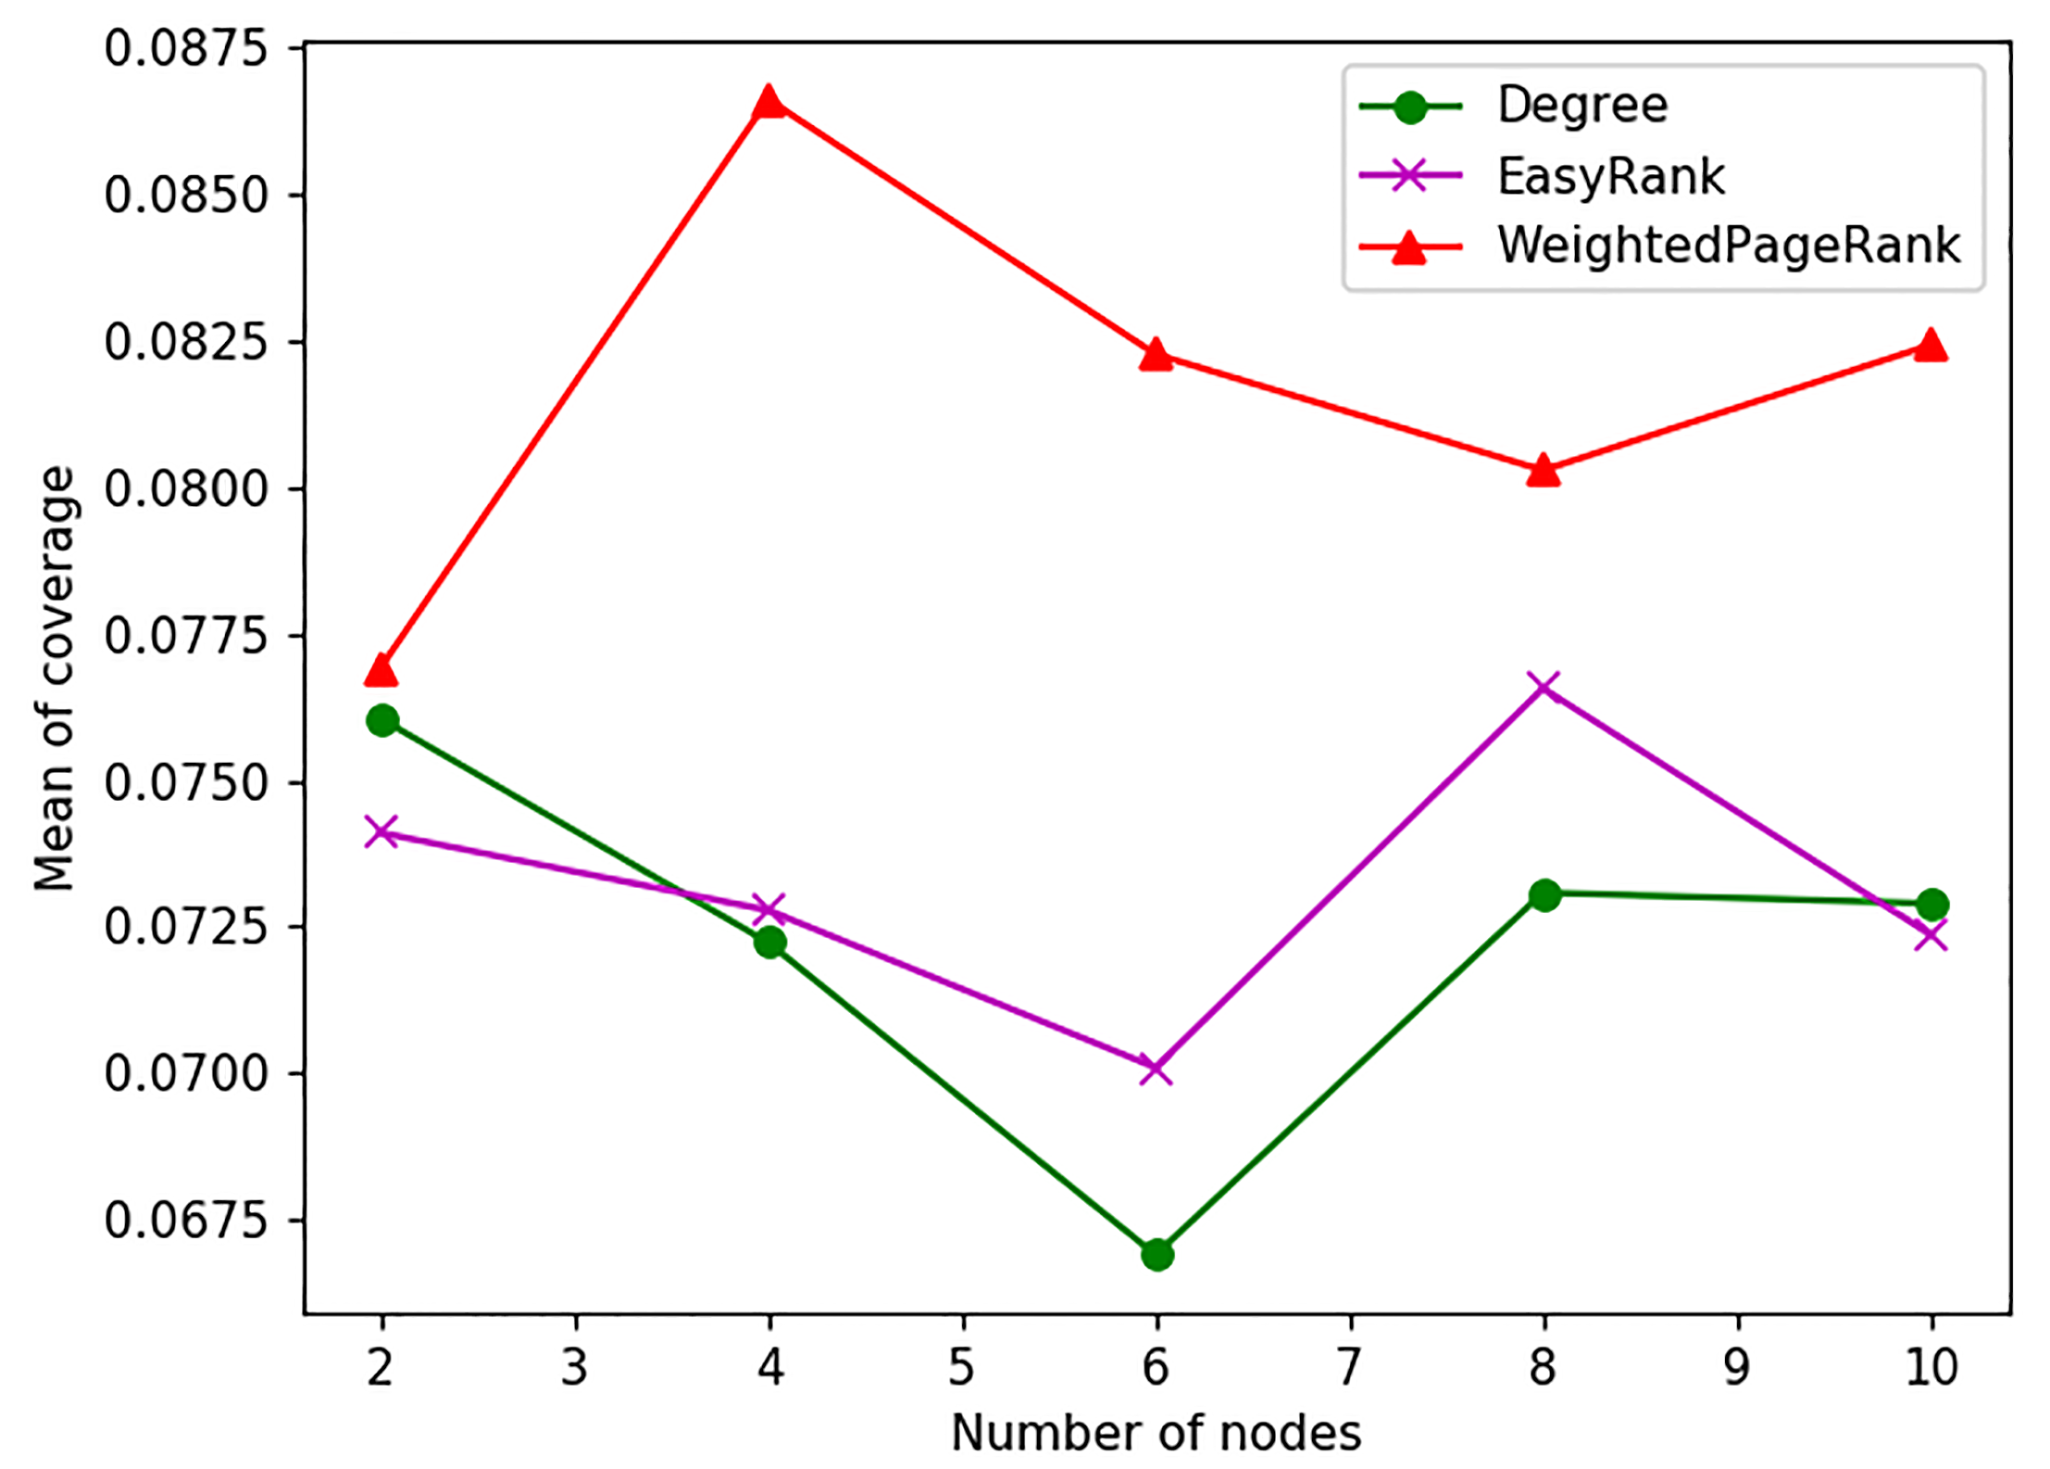
\includegraphics[width=0.9\textwidth]{imgs/Figure6.png}
    \caption{The mean of coverage}
\end{figure}
\column{0.5\textwidth}
imgs/Figure on the left shows a comparison of the mean of coverage under the condition of a fixed number of quotas. As the number of quotas is limited, the higher the mean of coverage rate, the better. The reason is that when some of these neighbors fail to provide services normally, nodes with higher average coverage rate have higher fault tolerance. In figure 6, the weighted PageRank approach achieves the best performance regarding the mean of coverage, as there are more nodes reaching the coverage rate requirement.
\end{columns}
\end{frame}

\begin{frame}{4. Evaluation}
\framesubtitle{Result Analysis}
\begin{columns}
\column{0.5\textwidth}
\begin{figure}
    \centering
    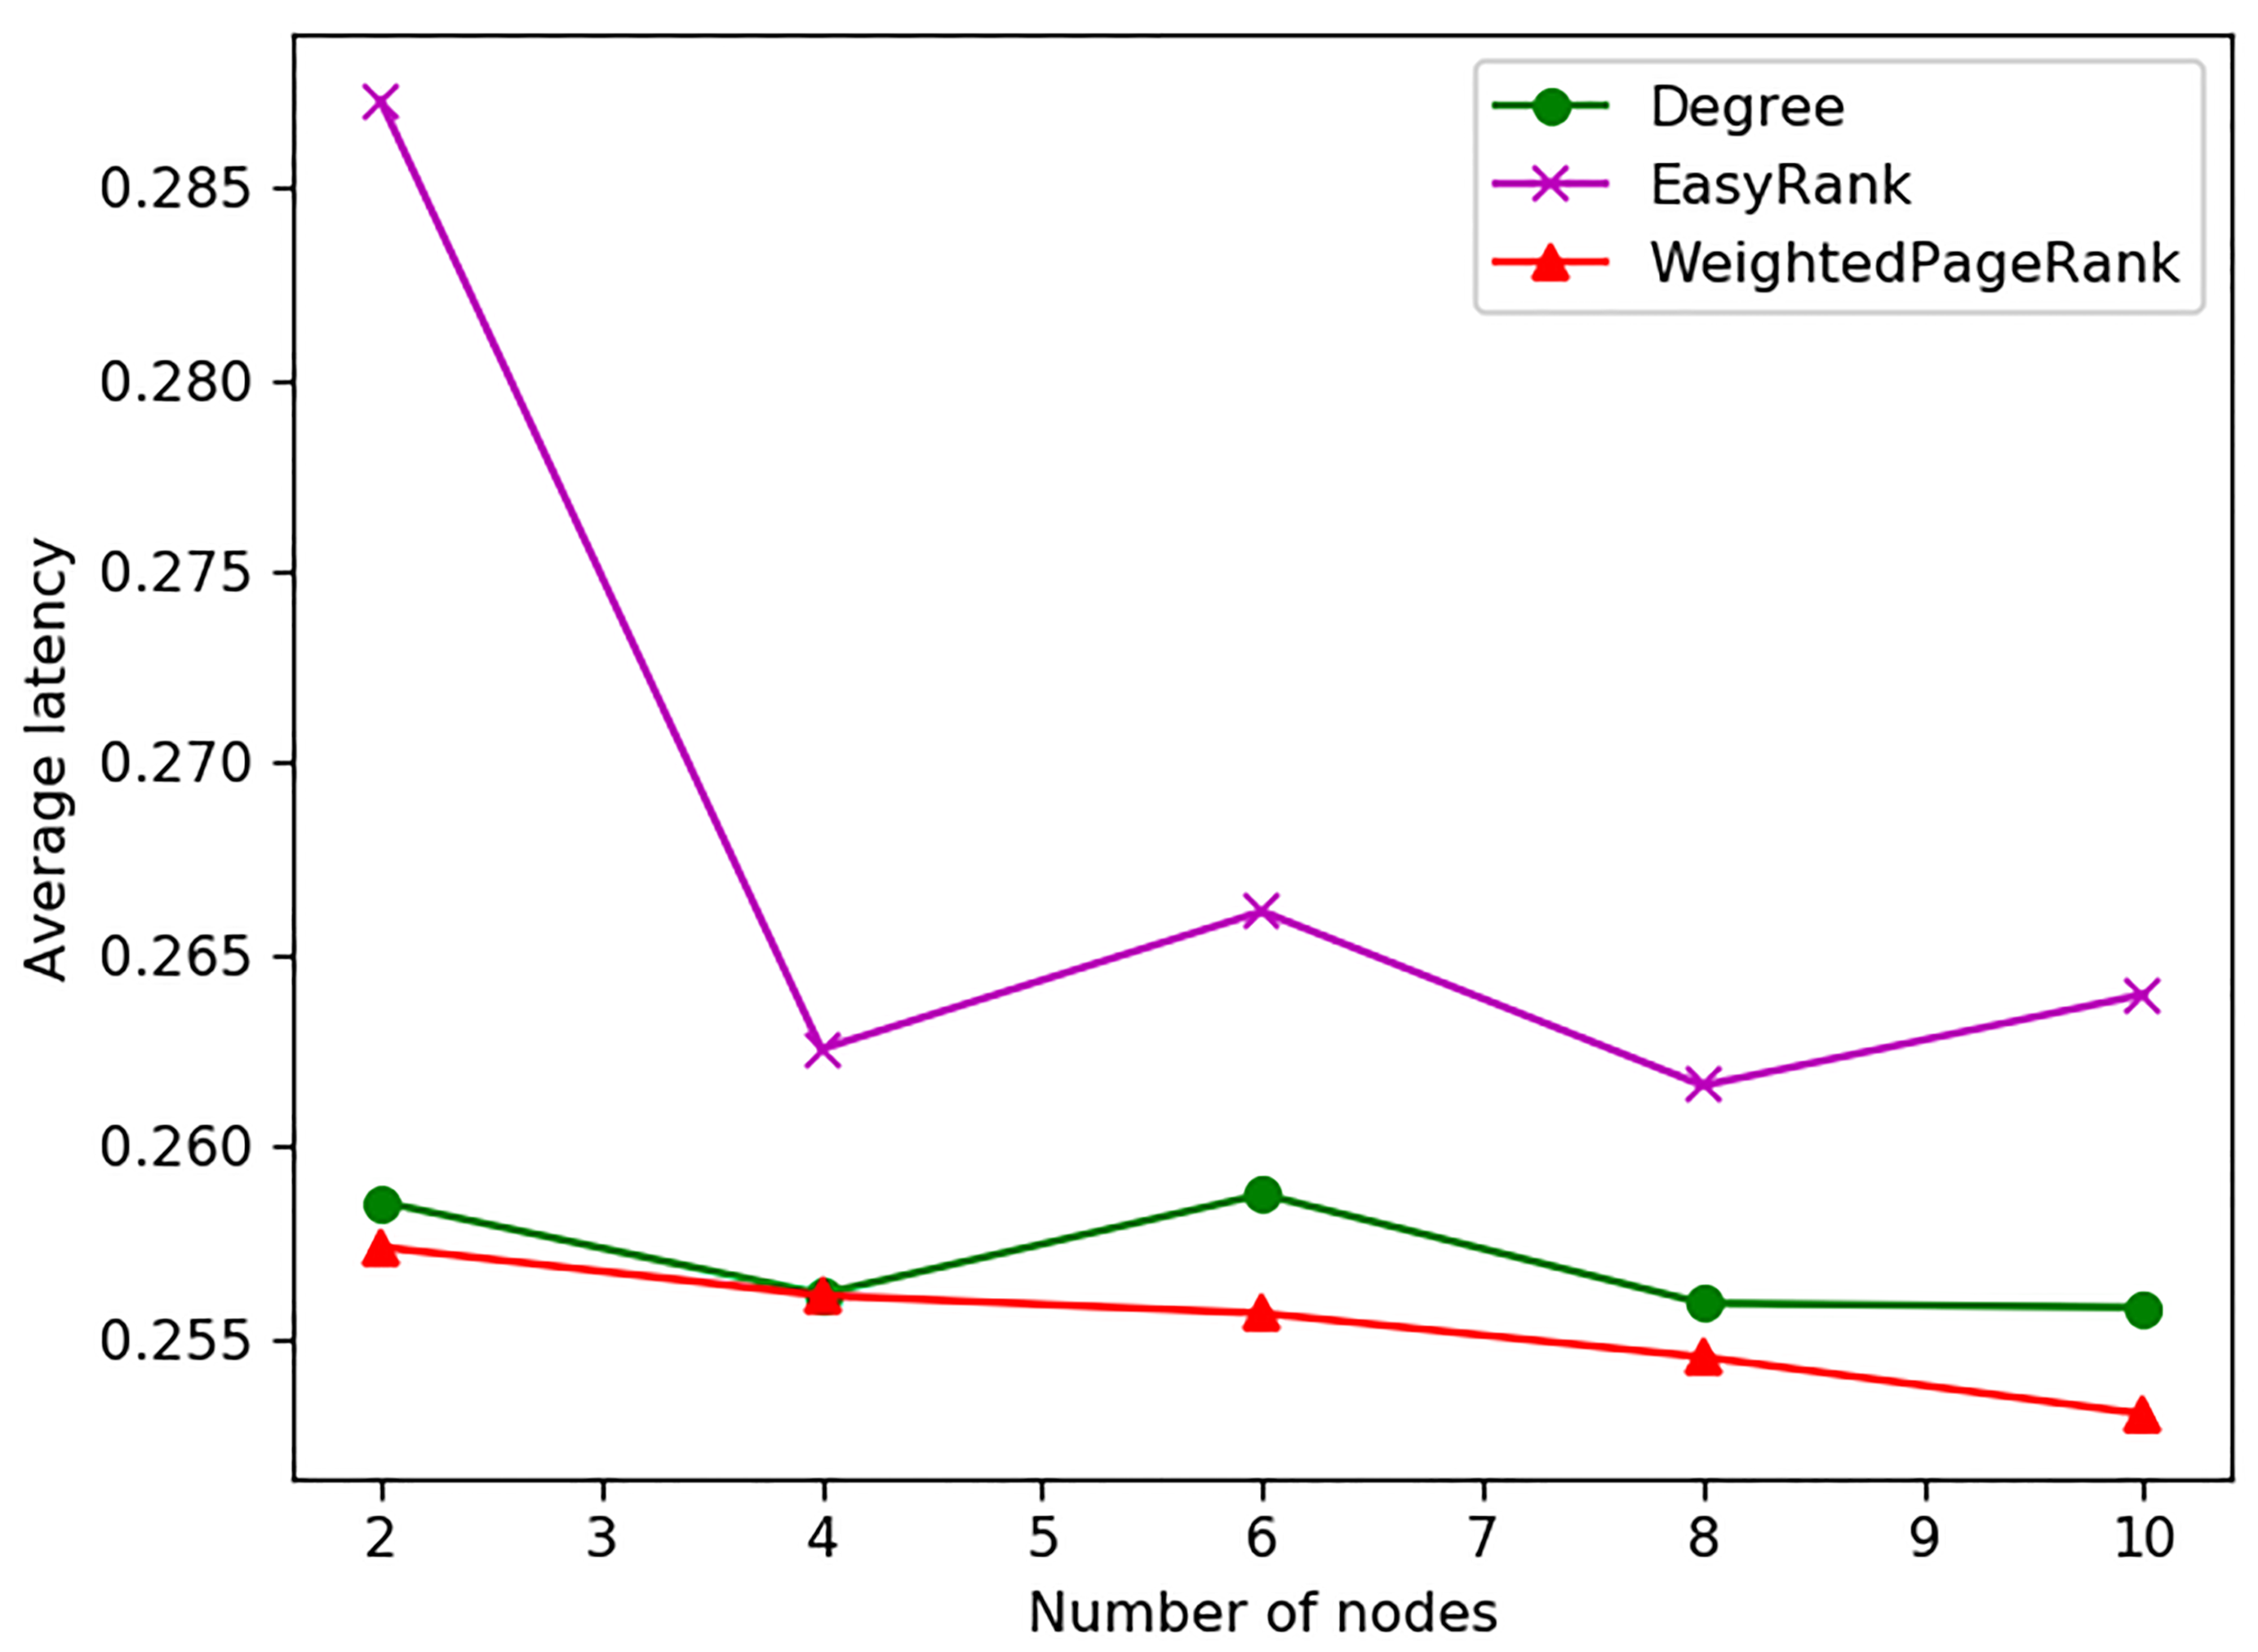
\includegraphics[width=0.9\textwidth]{imgs/Figure7.png}
    \caption{The average latency}
\end{figure}
\column{0.5\textwidth}
From the end-uses’ point of view, the service latency of the weighted PageRank method is the smallest compared to the other two methods. There are two main reasons for this. Firstly, the introduction of the bandwidth weights makes the selected node more bandwidth-intensive. Secondly, the weighted PageRank method has higher average coverage rate, so the service fault tolerance is better.
\end{columns}
\end{frame}

\begin{frame}{4. Evaluation}
\framesubtitle{Discussion}
Generally, there are tradeoffs between different measurements. The main goal is to enhance the service performance, alternatively, increase the number of nodes that meet the coverage requirements, while keeping other measurements improved. 20\% of nodes are randomly selected as users, whose requests follow the Poisson distribution. Through the simulation, the service rejection rate decreased by an average of 5.2\% in the case of high concurrent requests. Similar to the discussion in the mean of average section, nodes with higher average coverage rate have higher fault tolerance. Therefore, the service rejection rate will be reduced.
\end{frame}

\begin{frame}{Outline}
\begin{enumerate}[1. ]
\uncover<>{\item Introduction}
\uncover<>{\item Related Works}
\uncover<>{\item Content Dissemination Model}
\uncover<>{\item Evaluation}
\uncover<1>{\item Future Work}
\uncover<>{\item Conclusion}
\end{enumerate}
\end{frame}

\begin{frame}{5. Future Work}
Future work will mainly focus on two aspects:
\begin{itemize}
    \item \textbf{Edge network churn} brings about changes in network topology and content distribution.
    \item How to utilize the \textbf{edge intelligence} to enhance multiple services, for instance, content distribution, content-based computing, high-performance processing, is also an interesting subject we will focus on.
\end{itemize}
\end{frame}

\begin{frame}{Outline}
\begin{enumerate}[1. ]
\uncover<>{\item Introduction}
\uncover<>{\item Related Works}
\uncover<>{\item Content Dissemination Model}
\uncover<>{\item Evaluation}
\uncover<>{\item Future Work}
\uncover<1>{\item Conclusion}
\end{enumerate}
\end{frame}

\begin{frame}{6. Conclusion}
\begin{itemize}
    \item This paper proposes a decentralized PageRank-based content dissemination model in the edge of network. Our model solves the problem of how to effectively spread the content in the edge of network.
    \item The core of this model is a PageRank-based node selection algorithm in a decentralized manner to quantify the service capability of nodes for efficient caching.
    \item  Through the simulation, the service rejection rate decreased by an average of \textbf{5.2\%} in the case of high concurrent requests.
\end{itemize}
\end{frame}

\begin{frame}{Bonus}
\begin{figure}
    \centering
    
\includegraphics[width=0.9\textwidth]{imgs/journal.png}
    \caption{IJWSR}
\end{figure}
\end{frame}

\end{document}	% Done!